\documentclass[10pt,letter]{report}
\usepackage{import}
\import{../../../sistema/}{rutas}
\usepackage[T1]{fontenc}
%\usepackage[letterpaper, headsep=60pt, headheight=2cm]{geometry}
\usepackage{verbatim}
\usepackage[utf8x]{inputenc}
\usepackage[table]{xcolor}
\usepackage{float}
\usepackage{import}
\usepackage{textcomp}
\usepackage{ifthen}
\usepackage[spanish,mexico-com]{babel}
\usepackage{pdflscape}
\usepackage{mathrsfs}
\usepackage{amsmath}
\usepackage{amssymb}
\usepackage{bbm}
\usepackage{tikz}
\usepackage{fp}
\usepackage[autolanguage]{numprint}
\usepackage{array}
\usetikzlibrary{shapes}
\usepackage{subfigure}
\usepackage{ucs}
\usepackage[utf8x]{inputenc}
\usepackage{fontenc}
\usepackage{graphicx}
\usepackage{anysize}
\usepackage{relsize}
\usepackage{booktabs}

\usepackage{fancyhdr}
\usepackage[all]{xy}
\setlength{\headheight}{13.1pt}
\makeatletter\renewcommand\theenumi{\@alph\c@enumi}\makeatother
\renewcommand\labelenumi{\theenumi)}
\usepackage{amsthm}
\usepackage{enumerate}

\usepackage[]{mdframed}

\usepackage{marvosym}
\usepackage{tikzsymbols}
\usepackage{imakeidx}%for indexes
%\usepackage{tocbibind}
\usepackage{background}
\usepackage{titlesec}
\usepackage{multirow}
\usepackage{etoolbox}
\usepackage{fmtcount}
\usepackage{datetime}
\usepackage[bookmarks=true]{hyperref}%must be at the end of preamble
\usepackage[toc,section=subsection, acronym, shortcuts]{glossaries}
\usepackage[open,openlevel=0]{bookmark}
\usepackage{lipsum}
\usepackage{multicol}
\usepackage{wrapfig}
\usepackage[titletoc]{appendix}
\usepackage{sectsty}

\usepackage{titlesec}
\usepackage{pdfpages}
%---------------Formato Numeros \numprint-------------
\npdecimalsign{.}
\nprounddigits{2}
\npthousandsep{,}

%-----------------Espacio en blanco--------------------
\newcommand{\espacio}[1]{\vspace{#1}\begin{center}\textit{[EL RESTO DE ESTA PÁGINA HA SIDO DEJADO EN BLANCO\\
DE FORMA INTENCIONAL]}\end{center}\newpage}
\newcommand{\inserta}{\colorbox{principal}{\textcolor{orange}{Insertar}}}
\usepackage{textcomp}
\decimalpoint
%------------Diseño de página --------------------------------
\usepackage[centering, letterpaper,margin=2cm,top=1cm, headsep=24pt, headheight=2cm,includehead, includefoot]{geometry}

%------------Colores----------------------

\definecolor{principal}{RGB}{0, 53, 73}
\definecolor{secundario}{RGB}{43, 82, 96}
\definecolor{terciario}{RGB}{43,82,96}

%--------------Hipervinculos en color, ligas-azul, archivos-magenta, url-azul----------------
\hypersetup{
    colorlinks=true,
    linkcolor=secundario,
    filecolor=magenta,      
    urlcolor=blue}

%-------------Encabezado---------------------
\pagestyle{fancy}
\fancyhf{}

\chead{
\includegraphics[width=8cm]{\rutaImagenes/logo_valuami_fondo_blanco}}

%--------------Pie de página------------------
\cfoot{\textbf{\textcolor{principal}{\footnotesize{VALUAMI\tiny\textregistered}}}\\ \scriptsize{\textit{Amargura 50, Interior 7 y 8, Antigua Granada Parques de la Herradura.\\ Huixquilucan, Estado de M\'exico. CP 52786.\\ Tel. 52 94 76 80 / 55 89 96 34\\ \url{www.ami-mexico.com/valuami}}}}

%------------Títulos de seccion y subseccion--------------



%\renewcommand \thechapter {\Roman{chapter}}
\renewcommand \thesection {\Roman{section}}
%\renewcommand \thesubsection {\thesection.\arabic{subsection}}
%\renewcommand \thesubsubsection {\thesection.\arabic{subsection}.\arabic{subsubsection}}

\titleformat{\section}[hang]{\color{gray}\huge\bfseries}{\thesection.}{1em}{} 

%\chapterfont{\color{principal}}
\sectionfont{\color{principal}}
%\subsectionfont{\color{secundario}}
%\subsubsectionfont{\color{terciario}}

%------------------Profundidad del índice---------------------------

\setcounter{tocdepth}{3}
\setcounter{secnumdepth}{3}




%------------------Marca de agua---------------

\backgroundsetup{angle=0, contents={
\includegraphics[width=8cm]{\rutaImagenes/logo_valuami_fondo_blanco}},opacity=.3, scale=1}



%----------------------------Generales----------------------------
\newcommand{\tipoAvaluo}{insertar}
\newcommand{\bienesValuados}{insertar}%nombre del bien que se va a valuar
\newcommand{\lugarInforme}{insertar}

%--------------------Fechas---------------------------
\newcommand{\diainforme}{insertar} %dia del informe
\newcommand{\mesinforme}{insertar} %mes del informe
\newcommand{\annoinforme}{insertar} %año del informe

\newcommand{\diavalores}{insertar} %dia de valores
\newcommand{\mesvalores}{insertar} %mes de valores
\newcommand{\annovalores}{insertar} %año de valores

\newcommand{\diainspeccion}{insertar} %dia de inspeccion
\newcommand{\mesinspeccion}{insertar} %mes de inspeccion
\newcommand{\annoinspeccion}{insertar} %año de inspeccion

\newcommand{\fechaInforme}{\diainforme{} de \monthname[\mesinforme] de \annoinforme}
\newcommand{\fechaValores}{\diavalores{} de \monthname[\mesvalores] de \annovalores}
\newcommand{\fechaValoresCorto}{\diavalores/\mesvalores/\annovalores}
\newcommand{\fechaInspeccion}{\diainspeccion{} de \monthname[\mesinspeccion] de \annoinspeccion}

%----------------------------Perito Valuador---------------------
\newcommand{\peritoValuador}{insertar}
\import{\rutaValuatex/documentos_modelo/peritos/peritos/}{\peritoValuador}

%------------------------Perito Auxiliar-------------------
\newcommand{\peritoAuxiliar}{insertar}
\ifthenelse{\equal{\peritoAuxiliar}{n/a}}{ }{\import{\rutaValuatex/documentos_modelo/peritos/auxiliares/}{\peritoAuxiliar}}

%--------------Datos del solicitante-------------
\newcommand{\empresaSolicitante}{insertar}
\newcommand{\empresaCorto}{insertar}
\newcommand{\rfcEmpresa}{insertar}
\newcommand{\personaSolicitante}{insertar}
\newcommand{\caracterSolicitante}{insertar}

%--------------Datos del propietario-------------
\newcommand{\nombrePropietario}{insertar}

%-------------Vigencia----------------------------
\newcommand{\vigenciaInforme}{insertar}
\newcommand{\notaVigencia}{si}


%---------------Ubicacion del bien sujeto de valuaci\'on
\newcommand{\descripcionBien}{insertar}%en que consiste el bien que se va a valuar.
\newcommand{\ubicacionBien}{insertar}
\newcommand{\rfcBien}{insertar}

%------------Uso de la valuación---------------
\newcommand{\usoAvaluo}{insertar}
%--------------Desarrollo del avalúo en la especie-------------------
\newcommand{\EFde}{insertar}
\newcommand{\EFhasta}{insertar}
\newcommand{\EFdeHasta}{insertar}

%----------------Parámetros Peers--------------------------
%__________Multiplo________________
\newcommand{\peersa}{insertar}
\newcommand{\peersb}{insertar}
\newcommand{\peersc}{insertar}
\newcommand{\peersd}{insertar}
\newcommand{\peerse}{insertar}

%____________x veces________
\newcommand{\peersaTo}{insertar}
\newcommand{\peersbTo}{insertar}
\newcommand{\peerscTo}{insertar}
\newcommand{\peersdTo}{insertar}
\newcommand{\peerseTo}{insertar}

%___________Valor Múltiplo____________
\newcommand{\peersaMult}{insertar}
\newcommand{\peersbMult}{insertar}
\newcommand{\peerscMult}{insertar}
\newcommand{\peersdMult}{insertar}
\newcommand{\peerseMult}{insertar}

%___________Estadístico____________

\newcommand{\peersaEst}{insertar}
\newcommand{\peersbEst}{insertar}
\newcommand{\peerscEst}{insertar}
\newcommand{\peersdEst}{insertar}
\newcommand{\peerseEst}{insertar}

%============ WACC ===============
%---------------------- RF ------------------------------
\newcommand{\rfBase}{insertar}
\newcommand{\rfValor}{insertar}

%---------------------- Beta ----------------------------
\newcommand{\valorBeta}{insertar}
%-----------------------Premio de Mercado (ERP)----------------------------
\newcommand{\mercadoAccionario}{insertar}%mexicano o americano
\newcommand{\erpValor}{insertar}

%----------------------Riesgo Pais (CRP)-----------------
\newcommand{\crpValor}{insertar}

%-----------------------Costo de Capital (ke)--------------------
\newcommand{\keValor}{insertar}

%----------------------Costo de deuda (Kd)-----------------------
\newcommand{\kdValor}{insertar}

%----------------------- Valor Wacc----------------------------
\newcommand{\waccValor}{insertar}

%=============== DCF ======================
\newcommand{\periodoProyeccion}{insertar}
\newcommand{\proyCagr}{insertar}
\newcommand{\proyEbitMargin}{insertar}

\newcommand{\tasaFiscal}{insertar}
\newcommand{\reinvestmentRate}{insertar}


%============== RFR (Relief from royalties)==========
\newcommand{\tasaRegalias}{insertar}
\newcommand{\estadisticoTasaRegalias}{insertar}


%============== CIFRAS ======================
\newcommand{\valorDCF}{insertar}
\newcommand{\valorDCFLetra}{insertar} 

\newcommand{\valorPEERS}{insertar}
\newcommand{\valorPEERSLetra}{insertar} 

\newcommand{\valorFirma}{insertar}
\newcommand{\valorFirmaLetra}{insertar} 

\newcommand{\valorCapital}{insertar}
\newcommand{\valorCapitalLetra}{insertar} 

\newcommand{\valorRFR}{insertar}
\newcommand{\valorRFRLetra}{insertar} 

\newcommand{\valorResidual}{insertar}
\newcommand{\valorResidualLetra}{insertar} 

\newcommand{\valorActivoIntangible}{insertar}
\newcommand{\valorActivoIntangibleLetra}{insertar} 

\newcommand{\valorCapitalIntangible}{insertar}
\newcommand{\valorCApitalIntangibleLetra}{insertar} 

\newcommand{\moneda}{insertar}
\newcommand{\monedaCode}{insertar}









\makenoidxglossaries

%\import{\rutaValuatex/documentos_modelo/}{glosario}
%\import{\rutaValuatex/documentos_modelo/}{acronimos}
%\newglossaryentry{beta}
{
        name=Beta,
        description={El coeficiente Beta ($\beta$)} es una medida de volatilidad que estima el riesgo sistem\'atico de un activo.
}

\newglossaryentry{cashNeq}
{
        name=Cash \& Eq,
        description={Efectivo y equivalentes}
}

\newglossaryentry{efectivetaxrate}
{
        name=Effective Tax Rate,
        description={Tasa fiscal efectiva}
}

\newglossaryentry{enterprisevalue}
{
        name=Enterprise value,
        description={Valor de la empresa}
}

\newglossaryentry{equityvalue}
{
        name=Equity value,
        description={Valor del capital accionario}
}

\newglossaryentry{exitmultiple}
{
        name=Exit multiple,
        description={M\'ultiplo de salida}
}

\newglossaryentry{expdebt}
{
        name=Exp. Debt,
        description={Deuda expl\'icita}
}

\newglossaryentry{fairvalue}
{
        name=Fair Value,
        description={Valor razonable o valor justo de mercado}
}

\newglossaryentry{firmvalue}
{
        name=Firm Value,
        description={Valor de la firma o empresa}
}

\newglossaryentry{growthrate}
{
        name=Growth Rate,
        description={Tasa de crecimiento de ingresos netos}
}

\newglossaryentry{incomestatement}
{
        name=Income Statement,
        description={Estado de Resultados}
}

\newglossaryentry{investmentcapital}
{
        name=Investment Capital,
        description={Capital Invertido (IC)}
}

\newglossaryentry{leveredbeta}
{
        name=Levered beta,
        description={Beta apalancada}
}

\newglossaryentry{marketaproach}
{
        name=Market approach,
        description={Enfoque de mercado}
}

\newglossaryentry{netdebt}
{
        name=Net Debt,
        description={Deuda neta}
}

\newglossaryentry{nopat}
{
        name=Nopat,
        description={Flujo de Operaci\'on Neto}
}

\newglossaryentry{projectvaluation}
{
        name=Project Valuation,
        description={Valor razonable del proyecto de inversi\'on}
}

\newglossaryentry{riskfreerate}
{
        name=Risk Free Rate,
        description={Tasa Libre de Riesgo}
}

\newglossaryentry{sizeprime}
{
        name=Size Prime,
        description={Prima por tama\~no}
}

\newglossaryentry{terminalvalue}
{
        name=Terminal Value,
        description={Valor terminal}
}

\newglossaryentry{totaldebt}
{
        name=Total Debt,
        description={Deuda total}
}

\newglossaryentry{valuedrivers}
{
        name=Value drivers,
        description={Elevadores de Valor}
}
%\newacronym{cagr}{CAGR}{Tasa compuesta de crecimiento anual}
\newacronym{capm}{CAPM}{Modelo de Valoraci\'on de Activos de Capital}
\newacronym{chic}{CHIC}{Sociedades de Inversi\'on Cerradas}
\newacronym{crp}{CRP}{Riesgo Pa\'is}

\newacronym{dcf}{DCF}{Flujo de efectivo descontado (Discounted Cash FLow)}
\newacronym{erp}{ERP}{Premio de Mercado}
\newacronym{etr}{ETR}{Tasa Fiscal Efectiva}
\newacronym{fcff}{FCFF}{Flujo de efectivo libre a la Firma (Free Cash Flow to Firm)}
\newacronym{fcfe}{FCFE}{Flujo de efectivo libre al Capital (Free Cash Flow to Equity)}
\newacronym{g}{G}{Tasa de Crecimiento de ingresos netos (Grow Rate)}
\newacronym{ke}{Ke}{Costo de Capital Accionario}
\newacronym{kd}{Kd}{Costo de la deuda}
\newacronym{kpi}{KPI}{Indicador clave de desempe\~no o indicadores de gesti\'on \textit{(Key Performance Indicator)}}
\newacronym{mpeem}{MPEEM}{Multi-Period Excess Earnings Method}
\newacronym{nav}{NAV}{Valor neto de activos}
\newacronym{nca}{NCA}{Activo No Corriente}
\newacronym{nwc}{NWC}{Capital de Trabajo Neto}
\newacronym{peers}{PEERS}{M\'ultiplos de Cotizaci\'on}
\newacronym{rfr}{RFR}{M\'etodo de Flujo de Ahorro en Regalias}
\newacronym{wacc}{WACC}{Costo Promedio Ponderado de Capital}
\newacronym{wara}{WARA}{Costo Promedio Ponderado de Activos}

\usepackage{pdfpages}

\begin{document}

% Renombrar sección a inciso
\def\sectionautorefname{Inciso}
\def\subsectionautorefname{Inciso}


\thispagestyle{plain}
%
\includepdf[pages=-]{portada}

%-------------------------Índice-------------------------------
\newpage
\setcounter{page}{1}
\thispagestyle{fancy}
\tableofcontents

\newpage


\chapter{ANTECEDENTES.}\label{cap:1}
\thispagestyle{fancy}
%--------------------Datos del Valuador------------------
\section{DATOS DEL PERITO VALUADOR}\label{sec:a}
En \lugarInforme{} a los \numberstringnum{\diainforme} d\'ias del mes de \monthname[\mesinforme] del a\~no \numberstringnum{\annoinforme}, Yo, \textbf{\textcolor{principal}{\nombrePerito, \descripcionPerito}}, en mis funciones de PERITO VALUADOR, en uni\'on con mi perito auxiliar, \textcolor{principal}{\textbf{\nombreAuxiliar, \descripcionAuxiliar}}, con base en mis conocimientos t\'ecnicos y mediante la aplicaci\'on de t\'ecnicas de valuaci\'on seg\'un lo dispuesto por el art\'iculo 6, fracci\'on II, y dem\'as relativos de la Ley Federal de Corredur\'ia P\'ublica; art\'iculos 6, segundo p\'arrafo, 56 Bis del Reglamento de la Ley Federal de Corredur\'ia P\'ublica; expido a continuaci\'on el presente dictamen de avalúo de \textcolor{principal}{\tipoAvaluo}.\\







%------------------Datos del solicitante-----------------
\section{DATOS DEL SOLICITANTE}\label{sec:b}

The company \textcolor{principal}{\empresaSolicitante}, hereinafter referred to as \textcolor{principal}{``\empresaCorto''}, represented by \textcolor{principal}{\personaSolicitante} in his capacity as \textcolor{principal}{\caracterSolicitante}.



\espacio{3cm}

\chapter{DATOS DEL BIEN SUJETO DE VALUACI\'ON}\label{cap:2}
\thispagestyle{fancy}
\setcounter{section}{2}
%-----------------Datos del Propietario----------------
\section{DATOS DEL PROPIETARIO}\label{sec:c}}
\personaSolicitante.

%-----------------Tipo de servicio de valuación------
\section{TIPO DE SERVICIO DE VALUACI\'ON}\label{sec:d}
A petici\'on del solicitante se llev\'o a cabo un avalúo de \textcolor{principal}{\tipoAvaluo}.

%-----------------Vigencia-----------------------------
\section{VIGENCIA DEL INFORME}\label{sec:e}
%La vigencia del presente informe es de \textcolor{terciario}{\vigenciaInforme{} calendario}.\ifthenelse{\equal{\notaVigencia}{si}}{\footnote{A falta de disposici\'on expresa sobre la vigencia de este tipo de dict\'amenes de valuaci\'on, se tom\'o el plazo de 1 a\~no mencionado en el Art. 3 del Reglamento del C\'odigo Fiscal de la Federaci\'on.}}{ }\\[5pt]
%
%\textcolor{secundario}{Vigencia extr\'inseca o administrativa. }La vigencia de un aval\'uo est\'a determinada por su prop\'osito o destino y depender\'a de la temporabilidad que establezca en su caso la autoridad competente o instituci\'on administrativa que haga uso de dicho informe. \\[10pt]
%\textcolor{secundario}{Vigencia intr\'inseca. } Un informe conservar\'a su vigencia hasta en tanto no cambien de manera sustancial las condiciones y premisas fundamentales que dieron sustento al c\'alculo (\textit{ceteris paribus}); de tal manera que pudiera afectarse la fiabilidad de las cifras conclusivas de la estimaci\'on de valor.

El presente aval\'uo tiene vigencia de \textcolor{principal}{seis meses} a partir de la fecha de su emisi\'on, independientemente de las fechas de inicio y conclusi\'on del dictamen, en tanto no var\'ien las condiciones propias del Mercado o de la informaci\'on que el solicitante present\'o al suscrito para la elaboración del dictamen encomendado.




%---------------Descripción de los bienes Sujetos de valuación-----------
\section{DESCRIPCI\'ON DE LOS BIENES SUJETOS DE VALUACI\'ON}\label{sec:f}
\begin{enumerate}[1.]

\item Se tuvieron a la vista las obras artísticas objeto de valuaci\'on, mediante visita de inspecci\'on.
Adicionalmente, el solicitante entreg\'o al suscrito un reporte fotogr\'afico.
\item  El poseedor de las obras manifest\'o que la autor\'ia de las mismas se atribuye a (*)
\item \insertar cuenta con antecedentes sobre el origen de las obras.
\item \insertar cuenta con certificado de autenticidad de las obras.
\item \insertar cuenta con t\'itulo de propiedad que ampare la titularidad de la obra.

\end{enumerate}

\begin{table}[H]
\centering
\begin{tabular}{|c|m{.4\textwidth}|}
\hline
Obra& Dibujo	\\
\hline
Autor & Se atribuye a Ra\'ul Gonzalez Esquivel\\
\hline
T\'itulo & ``Figura S\'edente, Cultura Totonaca, Veracruz, Cl\'asico Tard\'io, Septiembre 29 de 1993'' \\
\hline
Tem\'atica & Representaci\'on de arte precolombino, im\'agenes de deidades, figuras antropomorfas, cabezas colosales, culto religioso ind\'igena y personajes mitol\'ogicos.\\
\hline
T\'ecnicas &Grafito sobre papel \\
\hline
Medidas & 41.5 cm $\times$ 59 cm \\
\hline
 Formato & Peque\~no \\
 \hline
 Firma & Se atribuye a Ra\'ul Gonzalez Esquivel \\
 \hline
 Fecha & Septiembre 29 de 1993. \\
 \hline
 Provenance & Colecci\'on particular\\
 \hline
 Certificado de autenticidad& Firmado por Pablo C. Goebel el 10 de abril de 1996.  \\
 \hline 
  Materiales empleados & Lapiz sobre papel\\
 \hline
 Caracter\'isticas especiales & Forma parte de una colecci\'on privada de 39 dibujos. 
Contiene dibujo con el texto ``Bufete Campos'' que corresponde a la obra por encargo. \\
\hline 
Ubicaci\'on & Calle Constituci\'on 124, colonia Centro, Veracruz, Veracruz, C.P. 91700.\\
\hline
\end{tabular}
\end{table}

\begin{table}[H]
\centering
\begin{tabular}{|c|m{.4\textwidth}|}
\hline
Obra& Dibujo	\\
\hline
Autor & Se atribuye a Ra\'ul Gonzalez Esquivel\\
\hline
T\'itulo & ``Dios Viejo (Remojadas, Estado de Veracruz). Cultura Totonaca. Septiembre 12 de 1993'' \\
\hline
Tem\'atica & Representaci\'on de arte precolombino, im\'agenes de deidades, figuras antropomorfas, cabezas colosales, culto religioso ind\'igena y personajes mitol\'ogicos.\\
\hline
T\'ecnicas &Grafito sobre papel \\
\hline
Medidas & 41.5 cm $\times$ 59 cm \\
\hline
 Formato & Peque\~no \\
 \hline
 Firma & Se atribuye a Ra\'ul Gonzalez Esquivel \\
 \hline
  Fecha & Septiembre 12 de 1993.\\
 \hline
 Provenance & Colecci\'on particular\\
 \hline
 Certificado de autenticidad& Firmado por Pablo C. Goebel el 10 de abril de 1996.  \\
 \hline 
  Materiales empleados & Lapiz sobre papel\\
 \hline
 Caracter\'isticas especiales & Forma parte de una colecci\'on privada de 39 dibujos. 
Contiene dibujo con el texto ``Bufete Campos'' que corresponde a la obra por encargo. \\
\hline 
Ubicaci\'on & Calle Constituci\'on 124, colonia Centro, Veracruz, Veracruz, C.P. 91700.\\
\hline

\end{tabular}
\end{table}

\begin{table}[H]
\centering
\begin{tabular}{|c|m{.4\textwidth}|}
\hline
Obra& Dibujo	\\
\hline
Autor & Se atribuye a Ra\'ul Gonzalez Esquivel\\
\hline
T\'itulo & ``Representaci\'on de Quetzalcoatl, Taj\'in, Ve. Cultura Totonaca. Septiembre 20 de 1993'.'' \\
\hline
Tem\'atica & Representaci\'on de arte precolombino, im\'agenes de deidades, figuras antropomorfas, cabezas colosales, culto religioso ind\'igena y personajes mitol\'ogicos.\\
\hline
T\'ecnicas &Grafito sobre papel \\
\hline
Medidas & 41.5 cm $\times$ 59 cm \\
\hline
 Formato & Peque\~no \\
 \hline
 Firma & Se atribuye a Ra\'ul Gonzalez Esquivel  \\
 \hline
 Fecha & Septiembre 20 de 1993. \\
 \hline
 Provenance & Colecci\'on particular\\
 \hline
 Certificado de autenticidad& Firmado por Pablo C. Goebel el 10 de abril de 1996.  \\
 \hline 
  Materiales empleados & Lapiz sobre papel\\
 \hline
 Caracter\'isticas especiales & Forma parte de una colecci\'on privada de 39 dibujos. 
Contiene dibujo con el texto ``Bufete Campos'' que corresponde a la obra por encargo. \\
\hline 
Ubicaci\'on & Calle Constituci\'on 124, colonia Centro, Veracruz, Veracruz, C.P. 91700.\\
\hline

\end{tabular}
\end{table}

\begin{table}[H]
\centering
\begin{tabular}{|c|m{.4\textwidth}|}
\hline
Obra& Dibujo	\\
\hline
Autor & Se atribuye a Ra\'ul Gonzalez Esquivel\\
\hline
T\'itulo & ``Nichos del edificio no. 16 del Taj\'in. El Taj\'in Veracruz. Septiembre 5 de 1993.''\\
\hline
Tem\'atica & Representaci\'on de arte precolombino, im\'agenes de deidades, figuras antropomorfas, cabezas colosales, culto religioso ind\'igena y personajes mitol\'ogicos.\\
\hline
T\'ecnicas &Grafito sobre papel \\
\hline
Medidas & 41.5 cm $\times$ 59 cm \\
\hline
 Formato & Peque\~no \\
 \hline
 Firma & Se atribuye a Ra\'ul Gonzalez Esquivel  \\
 \hline
  Fecha & Septiembre 5 de 1993.\\
 \hline
 Provenance & Colecci\'on particular\\
 \hline
 Certificado de autenticidad& Firmado por Pablo C. Goebel el 10 de abril de 1996.  \\
 \hline 
  Materiales empleados & Lapiz sobre papel\\
 \hline
 Caracter\'isticas especiales & Forma parte de una colecci\'on privada de 39 dibujos. 
Contiene dibujo con el texto ``Bufete Campos'' que corresponde a la obra por encargo. \\
\hline 
Ubicaci\'on & Calle Constituci\'on 124, colonia Centro, Veracruz, Veracruz, C.P. 91700.\\
\hline

\end{tabular}
\end{table}

\begin{table}[H]
\centering
\begin{tabular}{|c|m{.4\textwidth}|}
\hline
Obra& Dibujo	\\
\hline
Autor & Se atribuye a Ra\'ul Gonzalez Esquivel\\
\hline
T\'itulo & ``Cabeza de Anciano. Tres Zapotes, La Venta, Veracruz. Septiembre 11 de 1993.'' \\
\hline
Tem\'atica & Representaci\'on de arte precolombino, im\'agenes de deidades, figuras antropomorfas, cabezas colosales, culto religioso ind\'igena y personajes mitol\'ogicos.\\
\hline
T\'ecnicas &Grafito sobre papel \\
\hline
Medidas & 41.5 cm $\times$ 59 cm \\
\hline
 Formato & Peque\~no \\
 \hline
 Firma & Se atribuye a Ra\'ul Gonzalez Esquivel \\
 \hline
  Fecha & Septiembre 11 de 1993.\\
 \hline
 Provenance & Colecci\'on particular\\
 \hline
 Certificado de autenticidad& Firmado por Pablo C. Goebel el 10 de abril de 1996.  \\
 \hline 
  Materiales empleados & Lapiz sobre papel\\
 \hline
 Caracter\'isticas especiales & Forma parte de una colecci\'on privada de 39 dibujos. 
Contiene dibujo con el texto ``Bufete Campos'' que corresponde a la obra por encargo. \\
\hline 
Ubicaci\'on & Calle Constituci\'on 124, colonia Centro, Veracruz, Veracruz, C.P. 91700.\\
\hline

\end{tabular}
\end{table}

\begin{table}[H]
\centering
\begin{tabular}{|c|m{.4\textwidth}|}
\hline
Obra& Dibujo	\\
\hline
Autor & Se atribuye a Ra\'ul Gonzalez Esquivel\\
\hline
T\'itulo & `Èscultura Masculina S\'edente. El Zapotal, Mpio. de Ignacio de la Llave. S. VI-IX. Agosto 23 de 1993.'' \\
\hline
Tem\'atica & Representaci\'on de arte precolombino, im\'agenes de deidades, figuras antropomorfas, cabezas colosales, culto religioso ind\'igena y personajes mitol\'ogicos.\\
\hline
T\'ecnicas &Grafito sobre papel \\
\hline
Medidas & 41.5 cm $\times$ 59 cm \\
\hline
 Formato & Peque\~no \\
 \hline
 Firma &  Se atribuye a Ra\'ul Gonzalez Esquivel\\
 \hline
  Fecha & Agosto 23 de 1993. \\
 \hline
 Provenance & Colecci\'on particular\\
 \hline
 Certificado de autenticidad& Firmado por Pablo C. Goebel el 10 de abril de 1996.  \\
 \hline 
  Materiales empleados & Lapiz sobre papel\\
 \hline
 Caracter\'isticas especiales & Forma parte de una colecci\'on privada de 39 dibujos. 
Contiene dibujo con el texto ``Bufete Campos'' que corresponde a la obra por encargo. \\
\hline 
Ubicaci\'on & Calle Constituci\'on 124, colonia Centro, Veracruz, Veracruz, C.P. 91700.\\
\hline

\end{tabular}
\end{table}

\begin{table}[H]
\centering
\begin{tabular}{|c|m{.4\textwidth}|}
\hline
Obra& Dibujo	\\
\hline
Autor & Se atribuye a Ra\'ul Gonzalez Esquivel\\
\hline
T\'itulo & ``Mensajero del Sol. El Zapotal, Mpio. de Ignacio de la Llave. Cl\'asico Tard\'io. S. VI-IX D.C. Septiembre 03 de 1993.''\\
\hline
Tem\'atica & Representaci\'on de arte precolombino, im\'agenes de deidades, figuras antropomorfas, cabezas colosales, culto religioso ind\'igena y personajes mitol\'ogicos.\\
\hline
T\'ecnicas &Grafito sobre papel \\
\hline
Medidas & 41.5 cm $\times$ 59 cm \\
\hline
 Formato & Peque\~no \\
 \hline
 Firma & Se atribuye a Ra\'ul Gonzalez Esquivel \\
 \hline
  Fecha & Septiembre 3 de 1993.\\
 \hline
 Provenance & Colecci\'on particular\\
 \hline
 Certificado de autenticidad& Firmado por Pablo C. Goebel el 10 de abril de 1996.  \\
 \hline 
  Materiales empleados & Lapiz sobre papel\\
 \hline
 Caracter\'isticas especiales & Forma parte de una colecci\'on privada de 39 dibujos. 
Contiene dibujo con el texto ``Bufete Campos'' que corresponde a la obra por encargo. \\
\hline 
Ubicaci\'on & Calle Constituci\'on 124, colonia Centro, Veracruz, Veracruz, C.P. 91700.\\
\hline

\end{tabular}
\end{table}

\begin{table}[H]
\centering
\begin{tabular}{|c|m{.4\textwidth}|}
\hline
Obra& Dibujo	\\
\hline
Autor & Se atribuye a Ra\'ul Gonzalez Esquivel\\
\hline
T\'itulo & ``Sin t\'itulo, del Arq. Gonz\'alea Esquivel, aunque si muestra padre con hijo en sus brazos, o bien personaje con persona menor en brazos. Agosto 14 de 1993'' \\
\hline
Tem\'atica & Representaci\'on de arte precolombino, im\'agenes de deidades, figuras antropomorfas, cabezas colosales, culto religioso ind\'igena y personajes mitol\'ogicos.\\
\hline
T\'ecnicas &Grafito sobre papel \\
\hline
Medidas & 41.5 cm $\times$ 59 cm \\
\hline
 Formato & Peque\~no \\
 \hline
 Firma & Se atribuye a Ra\'ul Gonzalez Esquivel\\ 
 \hline
  Fecha &  Agosto 14 de 1993\\
 \hline
 Provenance & Colecci\'on particular\\
 \hline
 Certificado de autenticidad& Firmado por Pablo C. Goebel el 10 de abril de 1996.  \\
 \hline 
  Materiales empleados & Lapiz sobre papel\\
 \hline
 Caracter\'isticas especiales & Forma parte de una colecci\'on privada de 39 dibujos. 
Contiene dibujo con el texto ``Bufete Campos'' que corresponde a la obra por encargo. \\
\hline 
Ubicaci\'on & Calle Constituci\'on 124, colonia Centro, Veracruz, Veracruz, C.P. 91700.\\
\hline

\end{tabular}
\end{table}

\begin{table}[H]
\centering
\begin{tabular}{|c|m{.4\textwidth}|}
\hline
Obra& Dibujo	\\
\hline
Autor & Se atribuye a Ra\'ul Gonzalez Esquivel\\
\hline
T\'itulo & ``Dos cabezas, hombre y mujer, paga, Agosto 22 de 1993''\\
\hline
Tem\'atica & Representaci\'on de arte precolombino, im\'agenes de deidades, figuras antropomorfas, cabezas colosales, culto religioso ind\'igena y personajes mitol\'ogicos.\\
\hline
T\'ecnicas &Grafito sobre papel \\
\hline
Medidas & 41.5 cm $\times$ 59 cm \\
\hline
 Formato & Peque\~no \\
 \hline
 Firma & Se atribuye a Ra\'ul Gonzalez Esquivel\\ 
 \hline
  Fecha & Agosto 22 de 1993\\
 \hline
 Provenance & Colecci\'on particular\\
 \hline
 Certificado de autenticidad& Firmado por Pablo C. Goebel el 10 de abril de 1996.  \\
 \hline 
  Materiales empleados & Lapiz sobre papel\\
 \hline
 Caracter\'isticas especiales & Forma parte de una colecci\'on privada de 39 dibujos. 
Contiene dibujo con el texto ``Bufete Campos'' que corresponde a la obra por encargo. \\
\hline 
Ubicaci\'on & Calle Constituci\'on 124, colonia Centro, Veracruz, Veracruz, C.P. 91700.\\
\hline

\end{tabular}
\end{table}

\begin{table}[H]
\centering
\begin{tabular}{|c|m{.4\textwidth}|}
\hline
Obra& Dibujo	\\
\hline
Autor & Se atribuye a Ra\'ul Gonzalez Esquivel\\
\hline
T\'itulo & ``Tlalsolteotl, protectora de los partos y proporcionadora de los amores il\'icitos y las pasiones. Agosto de 1993.''\\
\hline
Tem\'atica & Representaci\'on de arte precolombino, im\'agenes de deidades, figuras antropomorfas, cabezas colosales, culto religioso ind\'igena y personajes mitol\'ogicos.\\
\hline
T\'ecnicas &Grafito sobre papel \\
\hline
Medidas & 41.5 cm $\times$ 59 cm \\
\hline
 Formato & Peque\~no \\
 \hline
 Firma & Se atribuye a Ra\'ul Gonzalez Esquivel\\ 
 \hline
  Fecha & Agosto de 1993.\\
 \hline
 Provenance & Colecci\'on particular\\
 \hline
 Certificado de autenticidad& Firmado por Pablo C. Goebel el 10 de abril de 1996.  \\
 \hline 
  Materiales empleados & Lapiz sobre papel\\
 \hline
 Caracter\'isticas especiales & Forma parte de una colecci\'on privada de 39 dibujos. 
Contiene dibujo con el texto ``Bufete Campos'' que corresponde a la obra por encargo. \\
\hline 
Ubicaci\'on & Calle Constituci\'on 124, colonia Centro, Veracruz, Veracruz, C.P. 91700.\\
\hline

\end{tabular}
\end{table}

\begin{table}[H]
\centering
\begin{tabular}{|c|m{.4\textwidth}|}
\hline
Obra& Dibujo	\\
\hline
Autor & Se atribuye a Ra\'ul Gonzalez Esquivel\\
\hline
T\'itulo & ``Dios Taj\'in, Dios de la lluvia y del trueno, edificio no. 5. Taj\'in Papantla, Veracruz. Septiembre de 1993.''\\
\hline
Tem\'atica & Representaci\'on de arte precolombino, im\'agenes de deidades, figuras antropomorfas, cabezas colosales, culto religioso ind\'igena y personajes mitol\'ogicos.\\
\hline
T\'ecnicas &Grafito sobre papel \\
\hline
Medidas & 41.5 cm $\times$ 59 cm \\
\hline
 Formato & Peque\~no \\
 \hline
 Firma & Se atribuye a Ra\'ul Gonzalez Esquivel\\ 
 \hline
  Fecha & Septiembre de 1993.\\
 \hline
 Provenance & Colecci\'on particular\\
 \hline
 Certificado de autenticidad& Firmado por Pablo C. Goebel el 10 de abril de 1996.  \\
 \hline 
  Materiales empleados & Lapiz sobre papel\\
 \hline
 Caracter\'isticas especiales & Forma parte de una colecci\'on privada de 39 dibujos. 
Contiene dibujo con el texto ``Bufete Campos'' que corresponde a la obra por encargo. \\
\hline 
Ubicaci\'on & Calle Constituci\'on 124, colonia Centro, Veracruz, Veracruz, C.P. 91700.\\
\hline

\end{tabular}
\end{table}

\begin{table}[H]
\centering
\begin{tabular}{|c|m{.4\textwidth}|}
\hline
Obra& Dibujo	\\
\hline
Autor & Se atribuye a Ra\'ul Gonzalez Esquivel\\
\hline
T\'itulo &``Carita SOnriente de los cerros. Cultura Totonaca (Veracruz). Mayo 15 de 1993.'' \\
\hline
Tem\'atica & Representaci\'on de arte precolombino, im\'agenes de deidades, figuras antropomorfas, cabezas colosales, culto religioso ind\'igena y personajes mitol\'ogicos.\\
\hline
T\'ecnicas &Grafito sobre papel \\
\hline
Medidas & 41.5 cm $\times$ 59 cm \\
\hline
 Formato & Peque\~no \\
 \hline
 Firma & Se atribuye a Ra\'ul Gonzalez Esquivel\\ 
 \hline
  Fecha & Mayo 15 de 1993.\\
 \hline
 Provenance & Colecci\'on particular\\
 \hline
 Certificado de autenticidad& Firmado por Pablo C. Goebel el 10 de abril de 1996.  \\
 \hline 
  Materiales empleados & Lapiz sobre papel\\
 \hline
 Caracter\'isticas especiales & Forma parte de una colecci\'on privada de 39 dibujos. 
Contiene dibujo con el texto ``Bufete Campos'' que corresponde a la obra por encargo. \\
\hline 
Ubicaci\'on & Calle Constituci\'on 124, colonia Centro, Veracruz, Veracruz, C.P. 91700.\\
\hline

\end{tabular}
\end{table}

\begin{table}[H]
\centering
\begin{tabular}{|c|m{.4\textwidth}|}
\hline
Obra& Dibujo	\\
\hline
Autor & Se atribuye a Ra\'ul Gonzalez Esquivel\\
\hline
T\'itulo & ``Carita Sonriente. Cultura Totonaca. Julio 19 de 1993.'' \\
\hline
Tem\'atica & Representaci\'on de arte precolombino, im\'agenes de deidades, figuras antropomorfas, cabezas colosales, culto religioso ind\'igena y personajes mitol\'ogicos.\\
\hline
T\'ecnicas &Grafito sobre papel \\
\hline
Medidas & 41.5 cm $\times$ 59 cm \\
\hline
 Formato & Peque\~no \\
 \hline
 Firma & Se atribuye a Ra\'ul Gonzalez Esquivel\\ 
 \hline
  Fecha & Julio 19 de 1993.\\
 \hline
 Provenance & Colecci\'on particular\\
 \hline
 Certificado de autenticidad& Firmado por Pablo C. Goebel el 10 de abril de 1996.  \\
 \hline 
  Materiales empleados & Lapiz sobre papel\\
 \hline
 Caracter\'isticas especiales & Forma parte de una colecci\'on privada de 39 dibujos. 
Contiene dibujo con el texto ``Bufete Campos'' que corresponde a la obra por encargo. \\
\hline 
Ubicaci\'on & Calle Constituci\'on 124, colonia Centro, Veracruz, Veracruz, C.P. 91700.\\
\hline

\end{tabular}
\end{table}

\begin{table}[H]
\centering
\begin{tabular}{|c|m{.4\textwidth}|}
\hline
Obra& Dibujo	\\
\hline
Autor & Se atribuye a Ra\'ul Gonzalez Esquivel\\
\hline
T\'itulo & `Hacha Votiva con Mono, Centro de Veracruz Post-Cl\'asico Tard\'io S. VI-IX D.C.''\\
\hline
Tem\'atica & Representaci\'on de arte precolombino, im\'agenes de deidades, figuras antropomorfas, cabezas colosales, culto religioso ind\'igena y personajes mitol\'ogicos.\\
\hline
T\'ecnicas &Grafito sobre papel \\
\hline
Medidas & 41.5 cm $\times$ 59 cm \\
\hline
 Formato & Peque\~no \\
 \hline
 Firma & Se atribuye a Ra\'ul Gonzalez Esquivel\\ 
 \hline
  Fecha & 6 de diciembre de 1993.\\
 \hline
 Provenance & Colecci\'on particular\\
 \hline
 Certificado de autenticidad& Firmado por Pablo C. Goebel el 10 de abril de 1996.  \\
 \hline 
  Materiales empleados & Lapiz sobre papel\\
 \hline
 Caracter\'isticas especiales & Forma parte de una colecci\'on privada de 39 dibujos. 
Contiene dibujo con el texto ``Bufete Campos'' que corresponde a la obra por encargo. \\
\hline 
Ubicaci\'on & Calle Constituci\'on 124, colonia Centro, Veracruz, Veracruz, C.P. 91700.\\
\hline

\end{tabular}
\end{table}

\begin{table}[H]
\centering
\begin{tabular}{|c|m{.4\textwidth}|}
\hline
Obra& Dibujo	\\
\hline
Autor & Se atribuye a Ra\'ul Gonzalez Esquivel\\
\hline
T\'itulo & ``Carita Sonriente de los Cerros. Cultura Totonaca (Veracruz). Mayo 8 de 1993.''\\
\hline
Tem\'atica & Representaci\'on de arte precolombino, im\'agenes de deidades, figuras antropomorfas, cabezas colosales, culto religioso ind\'igena y personajes mitol\'ogicos.\\
\hline
T\'ecnicas &Grafito sobre papel \\
\hline
Medidas & 41.5 cm $\times$ 59 cm \\
\hline
 Formato & Peque\~no \\
 \hline
 Firma & Se atribuye a Ra\'ul Gonzalez Esquivel\\ 
 \hline
  Fecha & Mayo 8 de 1993.\\
 \hline
 Provenance & Colecci\'on particular\\
 \hline
 Certificado de autenticidad& Firmado por Pablo C. Goebel el 10 de abril de 1996.  \\
 \hline 
  Materiales empleados & Lapiz sobre papel\\
 \hline
 Caracter\'isticas especiales & Forma parte de una colecci\'on privada de 39 dibujos. 
Contiene dibujo con el texto ``Bufete Campos'' que corresponde a la obra por encargo. \\
\hline 
Ubicaci\'on & Calle Constituci\'on 124, colonia Centro, Veracruz, Veracruz, C.P. 91700.\\
\hline

\end{tabular}
\end{table}

\begin{table}[H]
\centering
\begin{tabular}{|c|m{.4\textwidth}|}
\hline
Obra& Dibujo	\\
\hline
Autor & Se atribuye a Ra\'ul Gonzalez Esquivel\\
\hline
T\'itulo & ``Conjunto escult\'orico. Sacerdotes Portadores de un Incensario. Cultura Totonaca. Centro de Veracruz (Mixtequilla) Cl\'asico Tard\'io, S. VI-IX D.C.''\\
\hline
Tem\'atica & Representaci\'on de arte precolombino, im\'agenes de deidades, figuras antropomorfas, cabezas colosales, culto religioso ind\'igena y personajes mitol\'ogicos.\\
\hline
T\'ecnicas &Grafito sobre papel \\
\hline
Medidas & 41.5 cm $\times$ 59 cm \\
\hline
 Formato & Peque\~no \\
 \hline
 Firma & Se atribuye a Ra\'ul Gonzalez Esquivel\\ 
 \hline
  Fecha & \\
 \hline
 Provenance & Colecci\'on particular\\
 \hline
 Certificado de autenticidad& Firmado por Pablo C. Goebel el 10 de abril de 1996.  \\
 \hline 
  Materiales empleados & Lapiz sobre papel\\
 \hline
 Caracter\'isticas especiales & Forma parte de una colecci\'on privada de 39 dibujos. 
Contiene dibujo con el texto ``Bufete Campos'' que corresponde a la obra por encargo. \\
\hline 
Ubicaci\'on & Calle Constituci\'on 124, colonia Centro, Veracruz, Veracruz, C.P. 91700.\\
\hline

\end{tabular}
\end{table}

\begin{table}[H]
\centering
\begin{tabular}{|c|m{.4\textwidth}|}
\hline
Obra& Dibujo	\\
\hline
Autor & Se atribuye a Ra\'ul Gonzalez Esquivel\\
\hline
T\'itulo & ``Figura Sonriente. Pintada y articulada. El Zapotal. Mpio. Ignacio de la Llave, Cl\'asico Tard\'io S. VI-IX D.C.''\\
\hline
Tem\'atica & Representaci\'on de arte precolombino, im\'agenes de deidades, figuras antropomorfas, cabezas colosales, culto religioso ind\'igena y personajes mitol\'ogicos.\\
\hline
T\'ecnicas &Grafito sobre papel \\
\hline
Medidas & 41.5 cm $\times$ 59 cm \\
\hline
 Formato & Peque\~no \\
 \hline
 Firma & Se atribuye a Ra\'ul Gonzalez Esquivel\\ 
 \hline
  Fecha & \\
 \hline
 Provenance & Colecci\'on particular\\
 \hline
 Certificado de autenticidad& Firmado por Pablo C. Goebel el 10 de abril de 1996.  \\
 \hline 
  Materiales empleados & Lapiz sobre papel\\
 \hline
 Caracter\'isticas especiales & Forma parte de una colecci\'on privada de 39 dibujos. 
Contiene dibujo con el texto ``Bufete Campos'' que corresponde a la obra por encargo. \\
\hline 
Ubicaci\'on & Calle Constituci\'on 124, colonia Centro, Veracruz, Veracruz, C.P. 91700.\\
\hline

\end{tabular}
\end{table}

\begin{table}[H]
\centering
\begin{tabular}{|c|m{.4\textwidth}|}
\hline
Obra& Dibujo	\\
\hline
Autor & Se atribuye a Ra\'ul Gonzalez Esquivel\\
\hline
T\'itulo &``Carita Sonriente. Cultura Totonaca. Los Cerros, Veracruz. Cl\'asico Tard\'io S. VI-IX D.C. Octubre 8 de 1993.'' \\
\hline
Tem\'atica & Representaci\'on de arte precolombino, im\'agenes de deidades, figuras antropomorfas, cabezas colosales, culto religioso ind\'igena y personajes mitol\'ogicos.\\
\hline
T\'ecnicas &Grafito sobre papel \\
\hline
Medidas & 41.5 cm $\times$ 59 cm \\
\hline
 Formato & Peque\~no \\
 \hline
 Firma & Se atribuye a Ra\'ul Gonzalez Esquivel\\ 
 \hline
  Fecha & Octubre 8 de 1993.\\
 \hline
 Provenance & Colecci\'on particular\\
 \hline
 Certificado de autenticidad& Firmado por Pablo C. Goebel el 10 de abril de 1996.  \\
 \hline 
  Materiales empleados & Lapiz sobre papel\\
 \hline
 Caracter\'isticas especiales & Forma parte de una colecci\'on privada de 39 dibujos. 
Contiene dibujo con el texto ``Bufete Campos'' que corresponde a la obra por encargo. \\
\hline 
Ubicaci\'on & Calle Constituci\'on 124, colonia Centro, Veracruz, Veracruz, C.P. 91700.\\
\hline

\end{tabular}
\end{table}

\begin{table}[H]
\centering
\begin{tabular}{|c|m{.4\textwidth}|}
\hline
Obra& Dibujo	\\
\hline
Autor & Se atribuye a Ra\'ul Gonzalez Esquivel\\
\hline
T\'itulo & ``Figura Danzante. Cultura Totonaca, Veracruz. Octubre 08 de 1993.''\\
\hline
Tem\'atica & Representaci\'on de arte precolombino, im\'agenes de deidades, figuras antropomorfas, cabezas colosales, culto religioso ind\'igena y personajes mitol\'ogicos.\\
\hline
T\'ecnicas &Grafito sobre papel \\
\hline
Medidas & 41.5 cm $\times$ 59 cm \\
\hline
 Formato & Peque\~no \\
 \hline
 Firma & Se atribuye a Ra\'ul Gonzalez Esquivel\\ 
 \hline
  Fecha & Octubre 8 de 1993.\\
 \hline
 Provenance & Colecci\'on particular\\
 \hline
 Certificado de autenticidad& Firmado por Pablo C. Goebel el 10 de abril de 1996.  \\
 \hline 
  Materiales empleados & Lapiz sobre papel\\
 \hline
 Caracter\'isticas especiales & Forma parte de una colecci\'on privada de 39 dibujos. 
Contiene dibujo con el texto ``Bufete Campos'' que corresponde a la obra por encargo. \\
\hline 
Ubicaci\'on & Calle Constituci\'on 124, colonia Centro, Veracruz, Veracruz, C.P. 91700.\\
\hline

\end{tabular}
\end{table}

\begin{table}[H]
\centering
\begin{tabular}{|c|m{.4\textwidth}|}
\hline
Obra& Dibujo	\\
\hline
Autor & Se atribuye a Ra\'ul Gonzalez Esquivel\\
\hline
T\'itulo &``Carita Sonriente. Cultura Totonaca S. VI-XI D.C. Los Cerros, Veracruz. Octubre 08 de 1993.'' \\
\hline
Tem\'atica & Representaci\'on de arte precolombino, im\'agenes de deidades, figuras antropomorfas, cabezas colosales, culto religioso ind\'igena y personajes mitol\'ogicos.\\
\hline
T\'ecnicas &Grafito sobre papel \\
\hline
Medidas & 41.5 cm $\times$ 59 cm \\
\hline
 Formato & Peque\~no \\
 \hline
 Firma & Se atribuye a Ra\'ul Gonzalez Esquivel\\ 
 \hline
  Fecha & Octubre 8 de 1993.\\
 \hline
 Provenance & Colecci\'on particular\\
 \hline
 Certificado de autenticidad& Firmado por Pablo C. Goebel el 10 de abril de 1996.  \\
 \hline 
  Materiales empleados & Lapiz sobre papel\\
 \hline
 Caracter\'isticas especiales & Forma parte de una colecci\'on privada de 39 dibujos. 
Contiene dibujo con el texto ``Bufete Campos'' que corresponde a la obra por encargo. \\
\hline 
Ubicaci\'on & Calle Constituci\'on 124, colonia Centro, Veracruz, Veracruz, C.P. 91700.\\
\hline

\end{tabular}
\end{table}

\begin{table}[H]
\centering
\begin{tabular}{|c|m{.4\textwidth}|}
\hline
Obra& Dibujo	\\
\hline
Autor & Se atribuye a Ra\'ul Gonzalez Esquivel\\
\hline
T\'itulo & ``Carita Sonriente. Cultura Totonaca. S. VI-XI D.C. Los Cerros, Veracruz, Octubre 08 de 1993.'' \\
\hline
Tem\'atica & Representaci\'on de arte precolombino, im\'agenes de deidades, figuras antropomorfas, cabezas colosales, culto religioso ind\'igena y personajes mitol\'ogicos.\\
\hline
T\'ecnicas &Grafito sobre papel \\
\hline
Medidas & 41.5 cm $\times$ 59 cm \\
\hline
 Formato & Peque\~no \\
 \hline
 Firma & Se atribuye a Ra\'ul Gonzalez Esquivel\\ 
 \hline
  Fecha & Octubre 8 de 1993.\\
 \hline
 Provenance & Colecci\'on particular\\
 \hline
 Certificado de autenticidad& Firmado por Pablo C. Goebel el 10 de abril de 1996.  \\
 \hline 
  Materiales empleados & Lapiz sobre papel\\
 \hline
 Caracter\'isticas especiales & Forma parte de una colecci\'on privada de 39 dibujos. 
Contiene dibujo con el texto ``Bufete Campos'' que corresponde a la obra por encargo. \\
\hline 
Ubicaci\'on & Calle Constituci\'on 124, colonia Centro, Veracruz, Veracruz, C.P. 91700.\\
\hline

\end{tabular}
\end{table}

\begin{table}[H]
\centering
\begin{tabular}{|c|m{.4\textwidth}|}
\hline
Obra& Dibujo	\\
\hline
Autor & Se atribuye a Ra\'ul Gonzalez Esquivel\\
\hline
T\'itulo & ``Figura SOnriente Desnuda. El Zapotal. Mpio. de Ignacio de la Llave. Veracruz. Cultura Totonaca. Cl\'asico tard\'io. S. VI-IX D.C. Octubre 3 de 1993.''\\
\hline
Tem\'atica & Representaci\'on de arte precolombino, im\'agenes de deidades, figuras antropomorfas, cabezas colosales, culto religioso ind\'igena y personajes mitol\'ogicos.\\
\hline
T\'ecnicas &Grafito sobre papel \\
\hline
Medidas & 41.5 cm $\times$ 59 cm \\
\hline
 Formato & Peque\~no \\
 \hline
 Firma & Se atribuye a Ra\'ul Gonzalez Esquivel\\ 
 \hline
  Fecha & Octubree 3 de 1993.\\
 \hline
 Provenance & Colecci\'on particular\\
 \hline
 Certificado de autenticidad& Firmado por Pablo C. Goebel el 10 de abril de 1996.  \\
 \hline 
  Materiales empleados & Lapiz sobre papel\\
 \hline
 Caracter\'isticas especiales & Forma parte de una colecci\'on privada de 39 dibujos. 
Contiene dibujo con el texto ``Bufete Campos'' que corresponde a la obra por encargo. \\
\hline 
Ubicaci\'on & Calle Constituci\'on 124, colonia Centro, Veracruz, Veracruz, C.P. 91700.\\
\hline

\end{tabular}
\end{table}

\begin{table}[H]
\centering
\begin{tabular}{|c|m{.4\textwidth}|}
\hline
Obra& Dibujo	\\
\hline
Autor & Se atribuye a Ra\'ul Gonzalez Esquivel\\
\hline
T\'itulo & ``Figura S\'edente. Cultura Totonaca. El Salto. Mpio de Ignacio de la Llave. Veracruz. Octubre 4 de 1993.'' \\
\hline
Tem\'atica & Representaci\'on de arte precolombino, im\'agenes de deidades, figuras antropomorfas, cabezas colosales, culto religioso ind\'igena y personajes mitol\'ogicos.\\
\hline
T\'ecnicas &Grafito sobre papel \\
\hline
Medidas & 41.5 cm $\times$ 59 cm \\
\hline
 Formato & Peque\~no \\
 \hline
 Firma & Se atribuye a Ra\'ul Gonzalez Esquivel\\ 
 \hline
  Fecha & Octubre 4 de 1993. \\
 \hline
 Provenance & Colecci\'on particular\\
 \hline
 Certificado de autenticidad& Firmado por Pablo C. Goebel el 10 de abril de 1996.  \\
 \hline 
  Materiales empleados & Lapiz sobre papel\\
 \hline
 Caracter\'isticas especiales & Forma parte de una colecci\'on privada de 39 dibujos. 
Contiene dibujo con el texto ``Bufete Campos'' que corresponde a la obra por encargo. \\
\hline 
Ubicaci\'on & Calle Constituci\'on 124, colonia Centro, Veracruz, Veracruz, C.P. 91700.\\
\hline

\end{tabular}
\end{table}

\begin{table}[H]
\centering
\begin{tabular}{|c|m{.4\textwidth}|}
\hline
Obra& Dibujo	\\
\hline
Autor & Se atribuye a Ra\'ul Gonzalez Esquivel\\
\hline
T\'itulo & ``Figura Sonriente. Cultura Totonaca. Veracruz. Octubre 2 de 1993.'' \\
\hline
Tem\'atica & Representaci\'on de arte precolombino, im\'agenes de deidades, figuras antropomorfas, cabezas colosales, culto religioso ind\'igena y personajes mitol\'ogicos.\\
\hline
T\'ecnicas &Grafito sobre papel \\
\hline
Medidas & 41.5 cm $\times$ 59 cm \\
\hline
 Formato & Peque\~no \\
 \hline
 Firma & Se atribuye a Ra\'ul Gonzalez Esquivel\\ 
 \hline
  Fecha & Octubre 2 de 1993.\\
 \hline
 Provenance & Colecci\'on particular\\
 \hline
 Certificado de autenticidad& Firmado por Pablo C. Goebel el 10 de abril de 1996.  \\
 \hline 
  Materiales empleados & Lapiz sobre papel\\
 \hline
 Caracter\'isticas especiales & Forma parte de una colecci\'on privada de 39 dibujos. 
Contiene dibujo con el texto ``Bufete Campos'' que corresponde a la obra por encargo. \\
\hline 
Ubicaci\'on & Calle Constituci\'on 124, colonia Centro, Veracruz, Veracruz, C.P. 91700.\\
\hline

\end{tabular}
\end{table}

\begin{table}[H]
\centering
\begin{tabular}{|c|m{.4\textwidth}|}
\hline
Obra& Dibujo	\\
\hline
Autor & Se atribuye a Ra\'ul Gonzalez Esquivel\\
\hline
T\'itulo & ''Hacha Votiva con cara de guerrero. Diciembre 10 de 1993.'' \\
\hline
Tem\'atica & Representaci\'on de arte precolombino, im\'agenes de deidades, figuras antropomorfas, cabezas colosales, culto religioso ind\'igena y personajes mitol\'ogicos.\\
\hline
T\'ecnicas &Grafito sobre papel \\
\hline
Medidas & 41.5 cm $\times$ 59 cm \\
\hline
 Formato & Peque\~no \\
 \hline
 Firma & Se atribuye a Ra\'ul Gonzalez Esquivel\\ 
 \hline
  Fecha & Diciembre 10 de 1993. \\
 \hline
 Provenance & Colecci\'on particular\\
 \hline
 Certificado de autenticidad& Firmado por Pablo C. Goebel el 10 de abril de 1996.  \\
 \hline 
  Materiales empleados & Lapiz sobre papel\\
 \hline
 Caracter\'isticas especiales & Forma parte de una colecci\'on privada de 39 dibujos. 
Contiene dibujo con el texto ``Bufete Campos'' que corresponde a la obra por encargo. \\
\hline 
Ubicaci\'on & Calle Constituci\'on 124, colonia Centro, Veracruz, Veracruz, C.P. 91700.\\
\hline

\end{tabular}
\end{table}

\begin{table}[H]
\centering
\begin{tabular}{|c|m{.4\textwidth}|}
\hline
Obra& Dibujo	\\
\hline
Autor & Se atribuye a Ra\'ul Gonzalez Esquivel\\
\hline
T\'itulo & ``Hacha Votiva, representa a un guerrero muerto. Napatecuhtlan, Mpio. de Perote. Cl\'asico Tard\'io S. VI-IX. Diciembre 10 de 1993.'' \\
\hline
Tem\'atica & Representaci\'on de arte precolombino, im\'agenes de deidades, figuras antropomorfas, cabezas colosales, culto religioso ind\'igena y personajes mitol\'ogicos.\\
\hline
T\'ecnicas &Grafito sobre papel \\
\hline
Medidas & 41.5 cm $\times$ 59 cm \\
\hline
 Formato & Peque\~no \\
 \hline
 Firma & Se atribuye a Ra\'ul Gonzalez Esquivel\\ 
 \hline
  Fecha & Diciembre 10 de 1993.\\
 \hline
 Provenance & Colecci\'on particular\\
 \hline
 Certificado de autenticidad& Firmado por Pablo C. Goebel el 10 de abril de 1996.  \\
 \hline 
  Materiales empleados & Lapiz sobre papel\\
 \hline
 Caracter\'isticas especiales & Forma parte de una colecci\'on privada de 39 dibujos. 
Contiene dibujo con el texto ``Bufete Campos'' que corresponde a la obra por encargo. \\
\hline 
Ubicaci\'on & Calle Constituci\'on 124, colonia Centro, Veracruz, Veracruz, C.P. 91700.\\
\hline

\end{tabular}
\end{table}

\begin{table}[H]
\centering
\begin{tabular}{|c|m{.4\textwidth}|}
\hline
Obra& Dibujo	\\
\hline
Autor & Se atribuye a Ra\'ul Gonzalez Esquivel\\
\hline
T\'itulo & ``Tlasolteotl. Santana, Mpio. de Tlalixcoyan. Cl\'asico Tard\'io S. VI-IX D.C. Noviembre 26 de 1993.''\\
\hline
Tem\'atica & Representaci\'on de arte precolombino, im\'agenes de deidades, figuras antropomorfas, cabezas colosales, culto religioso ind\'igena y personajes mitol\'ogicos.\\
\hline
T\'ecnicas &Grafito sobre papel \\
\hline
Medidas & 41.5 cm $\times$ 59 cm \\
\hline
 Formato & Peque\~no \\
 \hline
 Firma & Se atribuye a Ra\'ul Gonzalez Esquivel\\ 
 \hline
  Fecha & Noviembre 26 de 1993. \\
 \hline
 Provenance & Colecci\'on particular\\
 \hline
 Certificado de autenticidad& Firmado por Pablo C. Goebel el 10 de abril de 1996.  \\
 \hline 
  Materiales empleados & Lapiz sobre papel\\
 \hline
 Caracter\'isticas especiales & Forma parte de una colecci\'on privada de 39 dibujos. 
Contiene dibujo con el texto ``Bufete Campos'' que corresponde a la obra por encargo. \\
\hline 
Ubicaci\'on & Calle Constituci\'on 124, colonia Centro, Veracruz, Veracruz, C.P. 91700.\\
\hline

\end{tabular}
\end{table}

\begin{table}[H]
\centering
\begin{tabular}{|c|m{.4\textwidth}|}
\hline
Obra& Dibujo	\\
\hline
Autor & Se atribuye a Ra\'ul Gonzalez Esquivel\\
\hline
T\'itulo & ``Cinuateteotl no. 2. El Cocuhite, Mpio. de Tlalixcoyan. Cl\'asico Tard\'io S. VI-IX D.C. Noviembre 27 de 1993.''\\
\hline
Tem\'atica & Representaci\'on de arte precolombino, im\'agenes de deidades, figuras antropomorfas, cabezas colosales, culto religioso ind\'igena y personajes mitol\'ogicos.\\
\hline
T\'ecnicas &Grafito sobre papel \\
\hline
Medidas & 41.5 cm $\times$ 59 cm \\
\hline
 Formato & Peque\~no \\
 \hline
 Firma & Se atribuye a Ra\'ul Gonzalez Esquivel\\ 
 \hline
  Fecha & Noviembre 27 de 1993.\\
 \hline
 Provenance & Colecci\'on particular\\
 \hline
 Certificado de autenticidad& Firmado por Pablo C. Goebel el 10 de abril de 1996.  \\
 \hline 
  Materiales empleados & Lapiz sobre papel\\
 \hline
 Caracter\'isticas especiales & Forma parte de una colecci\'on privada de 39 dibujos. 
Contiene dibujo con el texto ``Bufete Campos'' que corresponde a la obra por encargo. \\
\hline 
Ubicaci\'on & Calle Constituci\'on 124, colonia Centro, Veracruz, Veracruz, C.P. 91700.\\
\hline

\end{tabular}
\end{table}

\begin{table}[H]
\centering
\begin{tabular}{|c|m{.4\textwidth}|}
\hline
Obra& Dibujo	\\
\hline
Autor & Se atribuye a Ra\'ul Gonzalez Esquivel\\
\hline
T\'itulo & Cihuateteotl no.1, del Cocuhite, Mpio. de Tlalixcoyan. Cl\'asico Tard\'io. S. VI-IX. Noviembre 18 de 1998.''\\
\hline
Tem\'atica & Representaci\'on de arte precolombino, im\'agenes de deidades, figuras antropomorfas, cabezas colosales, culto religioso ind\'igena y personajes mitol\'ogicos.\\
\hline
T\'ecnicas &Grafito sobre papel \\
\hline
Medidas & 41.5 cm $\times$ 59 cm \\
\hline
 Formato & Peque\~no \\
 \hline
 Firma & Se atribuye a Ra\'ul Gonzalez Esquivel\\ 
 \hline
  Fecha & Noviembre 18 de 1993.\\
 \hline
 Provenance & Colecci\'on particular\\
 \hline
 Certificado de autenticidad& Firmado por Pablo C. Goebel el 10 de abril de 1996.  \\
 \hline 
  Materiales empleados & Lapiz sobre papel\\
 \hline
 Caracter\'isticas especiales & Forma parte de una colecci\'on privada de 39 dibujos. 
Contiene dibujo con el texto ``Bufete Campos'' que corresponde a la obra por encargo. \\
\hline 
Ubicaci\'on & Calle Constituci\'on 124, colonia Centro, Veracruz, Veracruz, C.P. 91700.\\
\hline

\end{tabular}
\end{table}

\begin{table}[H]
\centering
\begin{tabular}{|c|m{.4\textwidth}|}
\hline
Obra& Dibujo	\\
\hline
Autor & Se atribuye a Ra\'ul Gonzalez Esquivel\\
\hline
T\'itulo & ``Danzante. Centro de Veracruz. Cl\'asico Tard\'io S. VI-IX. Noviembre 10 de 1993.'' \\
\hline
Tem\'atica & Representaci\'on de arte precolombino, im\'agenes de deidades, figuras antropomorfas, cabezas colosales, culto religioso ind\'igena y personajes mitol\'ogicos.\\
\hline
T\'ecnicas &Grafito sobre papel \\
\hline
Medidas & 41.5 cm $\times$ 59 cm \\
\hline
 Formato & Peque\~no \\
 \hline
 Firma & Se atribuye a Ra\'ul Gonzalez Esquivel\\ 
 \hline
  Fecha & Noviembre 10 de 1993.\\
 \hline
 Provenance & Colecci\'on particular\\
 \hline
 Certificado de autenticidad& Firmado por Pablo C. Goebel el 10 de abril de 1996.  \\
 \hline 
  Materiales empleados & Lapiz sobre papel\\
 \hline
 Caracter\'isticas especiales & Forma parte de una colecci\'on privada de 39 dibujos. 
Contiene dibujo con el texto ``Bufete Campos'' que corresponde a la obra por encargo. \\
\hline 
Ubicaci\'on & Calle Constituci\'on 124, colonia Centro, Veracruz, Veracruz, C.P. 91700.\\
\hline

\end{tabular}
\end{table}

\begin{table}[H]
\centering
\begin{tabular}{|c|m{.4\textwidth}|}
\hline
Obra& Dibujo	\\
\hline
Autor & Se atribuye a Ra\'ul Gonzalez Esquivel\\
\hline
T\'itulo & ``Figura Sonriente Femenina. El Zapotal, Mpio. de Ignacio de la Llave. Cl\'asico Tard\'io S. VI-IX. Noviembre 13 de 1993.''\\
\hline
Tem\'atica & Representaci\'on de arte precolombino, im\'agenes de deidades, figuras antropomorfas, cabezas colosales, culto religioso ind\'igena y personajes mitol\'ogicos.\\
\hline
T\'ecnicas &Grafito sobre papel \\
\hline
Medidas & 41.5 cm $\times$ 59 cm \\
\hline
 Formato & Peque\~no \\
 \hline
 Firma & Se atribuye a Ra\'ul Gonzalez Esquivel\\ 
 \hline
  Fecha & Noviembre 13 de 1993. \\
 \hline
 Provenance & Colecci\'on particular\\
 \hline
 Certificado de autenticidad& Firmado por Pablo C. Goebel el 10 de abril de 1996.  \\
 \hline 
  Materiales empleados & Lapiz sobre papel\\
 \hline
 Caracter\'isticas especiales & Forma parte de una colecci\'on privada de 39 dibujos. 
Contiene dibujo con el texto ``Bufete Campos'' que corresponde a la obra por encargo. \\
\hline 
Ubicaci\'on & Calle Constituci\'on 124, colonia Centro, Veracruz, Veracruz, C.P. 91700.\\
\hline

\end{tabular}
\end{table}

\begin{table}[H]
\centering
\begin{tabular}{|c|m{.4\textwidth}|}
\hline
Obra& Dibujo	\\
\hline
Autor & Se atribuye a Ra\'ul Gonzalez Esquivel\\
\hline
T\'itulo & ``Jugador de Pelota. Mata Redonda, Mpio. de Villa Cuauht\'emoc. S. II-IX D.C. Periodo Panuco. Noviembre 1 de 1993.''\\
\hline
Tem\'atica & Representaci\'on de arte precolombino, im\'agenes de deidades, figuras antropomorfas, cabezas colosales, culto religioso ind\'igena y personajes mitol\'ogicos.\\
\hline
T\'ecnicas &Grafito sobre papel \\
\hline
Medidas & 41.5 cm $\times$ 59 cm \\
\hline
 Formato & Peque\~no \\
 \hline
 Firma & Se atribuye a Ra\'ul Gonzalez Esquivel\\ 
 \hline
  Fecha & Noviembre 1 de 1993.\\
 \hline
 Provenance & Colecci\'on particular\\
 \hline
 Certificado de autenticidad& Firmado por Pablo C. Goebel el 10 de abril de 1996.  \\
 \hline 
  Materiales empleados & Lapiz sobre papel\\
 \hline
 Caracter\'isticas especiales & Forma parte de una colecci\'on privada de 39 dibujos. 
Contiene dibujo con el texto ``Bufete Campos'' que corresponde a la obra por encargo. \\
\hline 
Ubicaci\'on & Calle Constituci\'on 124, colonia Centro, Veracruz, Veracruz, C.P. 91700.\\
\hline

\end{tabular}
\end{table}

\begin{table}[H]
\centering
\begin{tabular}{|c|m{.4\textwidth}|}
\hline
Obra& Dibujo	\\
\hline
Autor & Se atribuye a Ra\'ul Gonzalez Esquivel\\
\hline
T\'itulo & ``Tlasolteotl, con Gran Quechquemitl  Napiola, Mpio. de Tierra Blanca, Ver. Noviembre 03 de 1993.''\\
\hline
Tem\'atica & Representaci\'on de arte precolombino, im\'agenes de deidades, figuras antropomorfas, cabezas colosales, culto religioso ind\'igena y personajes mitol\'ogicos.\\
\hline
T\'ecnicas &Grafito sobre papel \\
\hline
Medidas & 41.5 cm $\times$ 59 cm \\
\hline
 Formato & Peque\~no \\
 \hline
 Firma & Se atribuye a Ra\'ul Gonzalez Esquivel\\ 
 \hline
  Fecha & Noviembre 3 de 1993.\\
 \hline
 Provenance & Colecci\'on particular\\
 \hline
 Certificado de autenticidad& Firmado por Pablo C. Goebel el 10 de abril de 1996.  \\
 \hline 
  Materiales empleados & Lapiz sobre papel\\
 \hline
 Caracter\'isticas especiales & Forma parte de una colecci\'on privada de 39 dibujos. 
Contiene dibujo con el texto ``Bufete Campos'' que corresponde a la obra por encargo. \\
\hline 
Ubicaci\'on & Calle Constituci\'on 124, colonia Centro, Veracruz, Veracruz, C.P. 91700.\\
\hline

\end{tabular}
\end{table}

\begin{table}[H]
\centering
\begin{tabular}{|c|m{.4\textwidth}|}
\hline
Obra& Dibujo	\\
\hline
Autor & Se atribuye a Ra\'ul Gonzalez Esquivel\\
\hline
T\'itulo & ``Hacha Votiva en forma de garza. Mpio de Coxquihui, VEracruz. Cla\'asico Tard\'io S. VI-IX D.C. Diciembre 10 de 1993.''\\
\hline
Tem\'atica & Representaci\'on de arte precolombino, im\'agenes de deidades, figuras antropomorfas, cabezas colosales, culto religioso ind\'igena y personajes mitol\'ogicos.\\
\hline
T\'ecnicas &Grafito sobre papel \\
\hline
Medidas & 41.5 cm $\times$ 59 cm \\
\hline
 Formato & Peque\~no \\
 \hline
 Firma & Se atribuye a Ra\'ul Gonzalez Esquivel\\ 
 \hline
  Fecha & Diciembre 10 de 1993.\\
 \hline
 Provenance & Colecci\'on particular\\
 \hline
 Certificado de autenticidad& Firmado por Pablo C. Goebel el 10 de abril de 1996.  \\
 \hline 
  Materiales empleados & Lapiz sobre papel\\
 \hline
 Caracter\'isticas especiales & Forma parte de una colecci\'on privada de 39 dibujos. 
Contiene dibujo con el texto ``Bufete Campos'' que corresponde a la obra por encargo. \\
\hline 
Ubicaci\'on & Calle Constituci\'on 124, colonia Centro, Veracruz, Veracruz, C.P. 91700.\\
\hline

\end{tabular}
\end{table}



%-----------------Ubicación del bien sujeto de valuavión
\section{UBICACI\'ON DE LOS BIENES SUJETOS DE VALUACI\'ON}\label{sec:g}
El lugar donde se encuentran los bienes sujetos de valuaci\'on es el ubicado en \textcolor{principal}{\ubicacionBien.}

%-----------------Propósito----------------------
\section{PROP\'OSITO DE LA VALUACI\'ON}\label{sec:h}
Estimar el valor de Mercado de \textcolor{principal}{una colecci\'on de treinta y siete litograf\'ias} para su presentaci\¡on en el juicio ejecutivo mercantil promovido por \insertar en contra de \insertar, registrado con el n\'umero de expediente 112/2020, radicado en el Juzgado Primero Mercantil del Distrito Judicial de Tlalnepantla, Estado de M\'exico.

La emisi\'on del presente dictamen valuatorio no representa un certificado de autenticidad de las obras objeto de valuaci\'on, por lo que su emisi\'on, distribuci\'on y/o reproducci\'on, de manera alguna puede entenderse como certificado de autenticidad y/o título de propiedad del solicitante.

%------------------Uso de la valuación---------------
\section{USO DE LA VALUACI\'ON}\label{sec:i}


The applicant has informed the Appraiser that they require this report for \textcolor{principal}{\usoAvaluo}.



\espacio{4cm}

\chapter{FUNDAMENTO JUR\'IDICO Y CONSIDERACIONES PREVIAS.}\label{cap:3}
\thispagestyle{fancy}
\setcounter{section}{9}

\section*{FUNDAMENTO JUR\'IDICO.}\label{sec:juridico}
El presente an\'alisis, as\'i como las opiniones y conclusiones del suscrito valuador fueron desarrolladas de conformidad con el art\'iculo 6 Fracci\'on II de la LFCP, el art\'iculo 56 bis de su reglamento, los lineamientos internacionales de valuaci\'on.\\

A continuaci\'on se mencionan diversos fundamentos de la normatividad mexicana que se relacionan con los informes de valuaci\'on:\\


\textcolor{principal}{Código de Comercio:}\\[10pt]

\textit{``Artículo 1252.- Los peritos deben tener título en la ciencia, arte, técnica, oficio o industria a que pertenezca la cuestión sobre la que ha de oírse su parecer, si la ciencia, arte, técnica, oficio o industria requieren título para su ejercicio.}\\[10pt]

\textit{Si no lo requirieran o requiriéndolo, no hubiere peritos en el lugar, podrán ser nombradas cualesquiera personas entendidas a satisfacción del juez, aun cuando no tengan título.}\\

\textit{La prueba pericial sólo será admisible cuando se requieran conocimientos especiales de la ciencia, arte, técnica, oficio o industria de que se trate, más no en lo relativo a conocimientos generales que la ley presupone como necesarios en los jueces, por lo que se desecharán de oficio aquellas periciales que se ofrezcan por las partes para ese tipo de conocimientos, o que se encuentren acreditadas en autos con otras pruebas, o tan sólo se refieran a simples operaciones aritméticas o similares.} \\[10pt] 

\textit{El título de habilitación de corredor público acredita para todos los efectos la calidad de perito valuador.''} (...)\\[10pt]

\textit{``Artículo 1257.- Los jueces podrán designar peritos de entre aquéllos autorizados como auxiliares de la administración de justicia por la autoridad local respectiva, o a solicitar que el perito sea propuesto por colegios, asociaciones o barras de profesionales, artísticas, técnicas o científicas o de las instituciones de educación superior públicas o privadas, o las cámaras de industria, comercio, o confederaciones de cámaras a la que corresponda al objeto del peritaje.  (...)''}\\[10pt]

\textit{``Artículo 1300.- Los avalúos harán prueba plena.}\\[10pt]


\textcolor{principal}{LEY FEDERAL DE CORREDUR\'IA P\'UBLICA}\\[10pt]

\textit{``ARTICULO 6o.- Al corredor público corresponde: (...)}\\[10pt]

\textit{II.- Fungir como perito valuador, para estimar, cuantificar y valorar los bienes, servicios, derechos y obligaciones que se sometan a su consideraci\'on, por nombramiento privado o por mandato de autoridad competente; (...)}\\[10pt]

\textit{VIII. Las dem\'as funciones que le señalen \'esta y otras leyes o reglamentos.}\\[10pt]

\textit{Las anteriores funciones se entender\'an sin perjuicio de lo dispuesto en otras leyes y no se consideran exclusivas de los corredores p\'ublicos.'' }\\[10pt]




\textcolor{principal}{REGLAMENTO DE LA LEY FEDERAL DE CORREDUR\'IA P\'UBLICA}\\


``\textcolor{secundario}{ARTICULO 56 Bis.-} \textit{El corredor p\'ublico en ejercicio de sus funciones como perito valuador, podr\'a estimar, cuantificar y valorar los bienes, servicios, derechos y obligaciones que se sometan a su consideraci\'on por nombramiento privado o por mandato de autoridad competente.} \\

\textit{El informe de valuaci\'on debe formularse de manera clara y objetiva, presentando el razonamiento y la informaci\'on suficiente con las cuales se obtiene el valor conclusivo del bien, servicio, derecho u obligaci\'on, y deber\'a contener cuando menos los siguientes rubros enunciativos: }

\begin{enumerate}[a)]

\item Nombre completo, n\'umero y plaza del Corredor as\'i como su firma y sello; 
\item Datos del solicitante; 
\item Datos del propietario, indicando en su caso la informaci\'on en que se basa; 
\item Tipo de servicio de valuaci\'on; 
\item Vigencia del aval\'uo, siendo este requisito obligatorio cuando exista una disposici\'on legal que as\'i lo establezca; 
\item Descripci\'on del bien, derecho, servicio u obligaci\'on materia del aval\'uo; 
\item  Cuando proceda, ubicaci\'on del bien materia de la valuaci\'on; 
\item Prop\'osito del informe de valuaci\'on; 
\item Uso del informe de valuaci\'on; 
\item Consideraciones previas a la valuaci\'on; 
\item Descripci\'on de enfoques de valuaci\'on aplicados; 
\item Fecha de la Inspecci\'on; 
\item En su caso fecha de referencia de valor; 
\item Fecha del informe de valuaci\'on; 
\item Fuentes de informaci\'on; 
\item Consideraciones previas a la conclusi\'on; 
\item Conclusi\'on de valor; 
\item Reporte fotogr\'afico, y 
\item En su caso, anexos. 

\end{enumerate}

\textit{Cualquier observaci\'on respecto a enfoques, fuentes de informaci\'on, elementos, limitaciones generales, entre otros, que incidan en la conclusi\'on del valor, deber\'an ser mencionadas en el informe.} \\

\textit{Cuando en raz\'on del servicio valuatorio, territorio, prop\'osito, uso u objeto del dictamen solicitado al corredor se desprenda que, con base en una normatividad particular expedida por autoridad competente que sea de car\'acter obligatorio, deba expedir o elaborar el dictamen utilizando leyes, normas, lineamientos, manuales o reglas espec\'ificas, el corredor podr\'a optar por sujetarse \'unicamente a dicha normatividad.} \\

\textit{Trat\'andose de remates, aval\'uos para efectos judiciales o procedimientos administrativos o aval\'uos solicitados por autoridades donde sea f\'isica o materialmente imposible realizar la inspecci\'on f\'isica del bien objeto de valuaci\'on, u obtener del solicitante o propietario la documentaci\'on correspondiente, se deber\'a se\~nalar expresamente en el dictamen y se realizar\'a el aval\'uo con los datos e informaci\'on de los que pueda allegarse el Corredor en el momento con los medios a su alcance.}''\\



\textcolor{principal}{AGREEMENT ESTABLISHING GUIDELINES FOR PUBLIC BROKERS TO ISSUE APPRAISALS ISSUED BY THE SECRETARY OF COMMERCE AND INDUSTRIAL PROMOTION, PUBLISHED IN THE OFFICIAL GAZETTE ON MARCH 9, 1999.}\\[10pt]



\textit{``Article 2.- The valuation report issued by the public broker shall be composed of the following sections:}

\begin{enumerate}[I.]

\item Background;
\item Data of the asset or service subject to valuation; 
\item Legal basis and preliminary considerations; 
\item  Methodology employed;
\item  Development of the appraisal, and
\item  Conclusions.

\end{enumerate}

\textit{Furthermore, in all cases, the public broker must have complete documentary support regarding the market study conducted for the purposes of the appraisal. (...)}\\[10pt]

\textit{Article 12.- In valuations performed by public brokers for intangible assets, considering their nature or type, their values may be determined as follows:}

\begin{enumerate}[I.-]
\item By researching the market for similar or substitute goods and products based on commercial references, implied and calculated values, considering sales volumes and profitability, possible purchase and sale cases, or alternatively, royalty payments for the use and exploitation of patents, trademarks, or franchises;

\item In the case of projects, an analysis will be conducted of the infrastructure of services available, marketing characteristics, technology used, price determination, investment costs, loss of profit, financial performance, and profit margins, in order to diagnose their investment margins, cash flows, and break-even points;

\item Through the study of the best utilization of projects and the commercial value of real or potential gross rents generated, as well as calculating the equivalent capital capable of providing those rents under non-inflationary and low-risk conditions, considering whether it is a project valuation or an ongoing business, or

\item When it comes to transfer pricing, it shall be done by applying the procedures established in the Income Tax Law or, alternatively, using the appropriate method for the case. (...)''

\end{enumerate}
%\textcolor{principal}{\textbf{PROCEDIMIENTO TECNICO PT-UE PARA LA ELABORACION DE TRABAJOS VALUATORIOS QUE PERMITAN DICTAMINAR EL VALOR DEL PATRIMONIO DE LAS UNIDADES ECONOMICAS.}}\\

1.- \textit{Introducci\'on (...)}\\

\textit{Premisas a la valuaci\'on de unidades econ\'omicas}\\
\begin{enumerate}[\indent\itshape a)]
\item \textit{Se analizan las unidades econ\'omicas como negocio en marcha} 
\item \textit{Se podr\'a valuar la unidad econ\'omica como un todo o las partes que la conforman}
\item \textit{Solamente pueden valuar unidades econ\'omicas peritos que cuenten con la especialidad valuatoria en negocios}
\item \textit{Se estima el valor comercial de unidades econ\'omicas}
\item \textit{Este procedimiento cumple en su desarrollo con los ocho pasos del proceso valuatorio establecidos en las metodolog\'ias y criterios de car\'acter t\'ecnico, considerando en todos los casos que existe una solicitud previa de trabajo valuatorio y se ha cumplido con el primer paso que consiste en la ``recepci\'on de solicitud''}
\item \textit{Todos los t\'erminos utilizados en este procedimiento se apegan al Glosario de T\'erminos de Valuaci\'on de Bienes Nacionales que emite el INDAABIN}
\item \textit{Todos los componentes y las acciones consideradas en este procedimiento, han sido incorporadas, vigilando que se apeguen al marco legal vigente}
\item \textit{La vigencia legal de los trabajos valuatorios elaborados bajo este procedimiento t\'ecnico, considera las condiciones f\'isicas, t\'ecnicas, econ\'omicas, pol\'iticas y sociales imperantes a la fecha de valores (...)} 
\end{enumerate}

\textit{\textcolor{principal}{1.4.14. Negocio en marcha}.- Es la entidad comercial que contin\'ua en operaci\'on en el futuro previsible. Por lo tanto, se supone que la empresa genera utilidades y que no tiene la intenci\'on ni la necesidad de liquidar o de reducir materialmente la escala de sus operaciones. Los negocios en marcha pueden valuarse mediante el enfoque basado en los costos, el enfoque de ingreso, o mediante el enfoque de comparativo de mercado.}\\

\textit{\textcolor{principal}{1.4.15. Unidad econ\'omica}.- Es un negocio con actividad econ\'omica realizada con el fin de obtener una ganancia, lucro o utilidad; se constituye por un conjunto de activos fijos (terrenos, construcciones, instalaciones, maquinaria, mobiliario y equipo), vinculados a activos intangibles e integrados conforme a un conjunto de tecnolog\'ias que le permiten producir bienes o prestar servicios en condiciones est\'andares de calidad y costo. A diferencia del negocio en marcha, la unidad econ\'omica puede tener o no utilidades; por lo tanto puede valuarse para operaci\'on continua o para liquidaci\'on. (...)}\\

\textit{\textcolor{principal}{1.4.19. Valor como negocio en marcha}.- El valor de una empresa que continua en operaci\'on en el futuro como un todo, sujeto a la utilidad o servicio potencial adecuado de la empresa, con todos sus activos y pasivos, plusval\'ia y potencialidades. Si la empresa es propietaria de las instalaciones que utiliza, \'estas forman parte del valor como negocio en marcha. El concepto implica la valuaci\'on de la empresa en operaci\'on continua.}\\

\textit{\textcolor{principal}{1.4.20. Valor de la unidad econ\'omica como negocio en marcha}.- Es el valor presente de los beneficios futuros esperados de la operaci\'on y desarrollo de la unidad econ\'omica atendiendo a posibles escenarios que toman en cuenta su ubicaci\'on, posici\'on tecnol\'ogica, capacidad instalada, vida \'util consumida, estado de conservaci\'on, potencial de ampliaci\'on y reconversi\'on, demanda de los bienes y/o servicios que produce y disponibilidad de los insumos, dentro de un horizonte de valuaci\'on y en el contexto y perspectivas de la econom\'ia en que se desempe\~na. Existir\'an tantos valores de la unidad econ\'omica como negocio en marcha como escenarios factibles puedan ser planteados. El valor de la unidad econ\'omica como negocio en marcha puede utilizarse para determinar el valor conclusivo de acuerdo al Uso, Prop\'osito y Finalidad del aval\'uo. (...)}\\

\textit{\textcolor{principal}{2.7.3. Evaluaci\'on financiera}.- Una vez que se ha determinado el flujo de efectivo libre, se debe definir la tasa de descuento bajo la cual \'este se ha de descontar a valor presente; para ello el valuador de bienes nacionales debe definir la tasa de descuento de acuerdo al objetivo del estudio, utilizando distintos m\'etodos financieros generalmente aceptados, como pueden ser: el Modelo para la Valoraci\'on de los Activos de Capital (CAPM, por sus siglas en ingl\'es), Teor\'ia de Fijaci\'on de Precios por Arbitraje, el Costo de Capital Promedio Ponderado (CPC o WACC de sus siglas en ingl\'es1), Costo del Capital por Comparables de Negocios del mismo Sector, entre otros.}\\
\textit{O bien, el valuador de bienes nacionales puede referirse al procedimiento t\'ecnico PT-TD para la obtenci\'on de tasas de descuento.}\\
\textit{Al final del horizonte de valuaci\'on se debe establecer el valor residual del negocio, considerando en algunos casos un valor continuo del negocio, asumiendo su operaci\'on a perpetuidad, o en otros, considerando el valor de rescate de los activos menos los costos de cierre de la unidad econ\'omica. El valor residual se aplica siempre y cuando la naturaleza de la unidad econ\'omica lo requiera y debe determinarse mediante principios financieros generalmente aceptados.}\\

\textit{\textcolor{principal}{2.7.4. Valor de la unidad econ\'omica}.- El resultado obtenido mediante el modelo financiero es el valor presente neto, el cual representa el valor del negocio.}\\
\textit{A partir del valor del negocio, se determina el valor de la unidad econ\'omica restando el valor de los pasivos financieros (deuda con bancos, proveedores con costo, deuda subordinada, acciones preferentes, entre otros), sumando el valor de los activos circulantes l\'iquidos o disponibles (normalmente caja e inversiones temporales y en algunos casos cuentas de inventarios no considerados en los flujos de efectivo) y de los bienes no operativos (bienes no utilizados en la operaci\'on de la unidad econ\'omica), y por otro lado restando los pasivos contingentes (ambientales, laborales, legales, entre otros). Este proceso se muestra de manera esquem\'atica a trav\'es de la siguiente figura:}\\

\begin{figure}[H]
\centering

\includegraphics[width=10cm]{\rutaValuatex/sistema/imagenes/pt-ue}
\end{figure}

\textit{\textcolor{principal}{2.8. Estimaci\'on final del valor}.- El valuador de bienes nacionales de negocios en marcha, debe estimar el valor de la unidad econ\'omica como negocio en marcha en funci\'on del Uso, Prop\'osito y Finalidad del trabajo y dictamen valuatorio. (...)''}\\


\espacio{1cm}

%---------------Consideraciones previas a la valuaci\'on--------------------
\section{CONSIDERACIONES PREVIAS A LA VALUACI\'ON}\label{sec:j}

	\subsection{Condiciones, restricciones y limitantes del informe}
	\begin{enumerate}[\indent a)]

\item Se deja constancia que la valuaci\'on solicitada, ha sido elaborada considerando que la informaci\'on y documentaci\'on puesta a mi disposici\'on directamente por el solicitante o a trav\'es de los sitios de Internet consultados en relaci\'on con el bien a valuar.

\item La informaci\'on proporcionada es considerada por el solicitante como confiable, veraz y fidedigna de acuerdo a manifestaciones que, bajo protesta de decir verdad, fue entregada al suscrito.

\item No se tiene conocimiento de sucesos que pueden afectar en modo alguno el objeto de la valuaci\'on encomendada y que no se hayan dado a conocer en los mismos.

\item Por otra parte, el suscrito deja constancia de que, fuera del informaci\'on y documentaci\'on puesta a mi disposici\'on por el solicitante, no se tiene conocimiento ni informaci\'on revelada adicional a la antes detallada, ni tampoco fueron revelados o puestos a mi disposici\'on documentos o informaciones distintas a las descritas con anterioridad.

\item Asimismo, se deja constancia que, con fecha  \textcolor{principal}{\fechaInspeccion}, el suscrito Corredor P\'ublico llev\'o a cabo la visita de inspecci\'on de las obras objeto del presente aval\'uo, mismas que se realiz\'o en el domicilio ubicado en\textcolor{principal}{\direccionSolicitante}, lugar en el que fui atendido por \insertar, quien dijo ser propietario y/o poseedor de los bienes valuados.

\item El solicitante podr\'a utilizar los datos contenidos en el presente dictamen para los fines que le sean convenientes, sin restricción legal para su uso, distribuci\'on o publicaci\'on

\item No obstante lo anterior, se hace constar que el aval\'uo encomendado no representa un certificado de autenticidad de las obras objeto de valuaci\'on, por lo que su emisi\'on, distribuci\'on y/o reproducci\'on, de manera alguna puede entenderse como certificado de autenticidad y/o t\'itulo de propiedad del solicitante.

\item Los an\'alisis, opiniones utilizadas y las conclusiones presentadas en este trabajo parten de la experiencia, capacidad y criterios profesionales del suscrito, as\'i como de las disposiciones legales aplicables y las declaraciones y suposiciones especiales manifestadas por el solicitante del presente aval\'uo.

\item Manifiesto que no tengo ning\'un inter\'es en el bien objeto del presente aval\'uo, por lo que emito mi opini\'on de valor con plena independencia y sin ning\'un inter\'es que implique parcialidad.
Asimismo, se hace constar que el presente dictamen se emite con base en las manifestaciones e informaci\'on proporcionadas por el solicitante, liberando al suscrito de cualquier responsabilidad de naturaleza civil o penal, pues no se prejuzga respecto de la autenticidad de los documentos exhibidos e informaci\'o n proporcionada, as\'i como de la propiedad del bien materia de valuaci\'on.


\end{enumerate}
	%
\begin{enumerate}[\indent\itshape 2.1.]
\item \textcolor{principal}{\textit{Valor de mercado. }}

\textit{Cuant\'ia estimada por la que un bien o activo, o pasivo deber\'ia intercambiarse en la fecha de valuaci\'on entre un comprador dispuesto a comprar y un vendedor dispuesto a vender, en una transacci\'on libre, tras una comercializaci\'on adecuada en las que las partes hayan actuado con conocimiento, de manera prudente y sin coacci\'on.''}

\item \textcolor{principal}{\textit{Valor razonable.} }

\textit{Precio estimado para la transacci\'on de un bien o activo, o pasivo entre dos partes identificadas, informadas y dispuestas que refleja los intereses respectivos de dichas partes. }\\

\textit{Esta definici\'on no es aplicable en el caso de valuaciones para uso en la elaboraci\'on de estados financieros, ver 5.1.''}

\item  \textcolor{principal}{\textit{Precio, Costo y Valor. }}

\begin{enumerate}[\indent\itshape 2.\theenumi.1.]
\item \textcolor{principal}{\textit{Precio. }}

\textit{Es la cantidad expresada en unidades monetarias, ofrecida o pagada por un bien o activo. Debido a la capacidad financiera, motivaci\'on o intereses especiales de un comprador o vendedor dado, el precio pagado pue de ser diferente del valor que podr\'ia asignarse a los bienes y servicios por otros.''}

\item  \textcolor{principal}{\textit{Costo .}}

\textit{Es la cantidad expresada en unidades monetarias requerida para crear o producir el bien o activo. Cuando ese bien o activo ha sido completado, su costo es un hecho. El precio se relaciona con el costo puesto que el precio pagado por un bien o servicio se convierte en su costo para el comprador.''}

\item \textcolor{principal}{ \textit{Valor. }}

\textit{Es una opini\'on de: }
\begin{enumerate}[\indent\itshape a)]

\item\textit{ El precio m\'as probable que habr\'ia de pagarse por un bien o activo en un intercambio, o;} 
\item \textit{Los beneficios econ\'omicos de tener en propiedad esos bienes o activos.''}

\end{enumerate}
\end{enumerate}

\item  \textcolor{principal}{\textit{Valor Comercial. }}

\textit{Valor Comercial el precio estimado y m\'as probable, por el cual una propiedad se intercambiar\'ia en la fecha del avalu\'o, entre un comprador y un vendedor actuando por voluntad propia en una transacci\'on sin intermediarios, con un plazo razonable de exposici\'on donde ambas partes act\'uan con conocimiento de los hechos pertinentes, con prudencia y sin compulsi\'on.''}\\

\textit{As\'i mismo, es importante aclarar que para efectos del presente dictamen deber\'a entenderse por Inversiones de Terreno a todas aquellas inversiones y preparaciones necesarias para el desarrollo de proyectos con el m\'aximo y mejor uso que presentan los inmuebles, mismo que dan plusval\'ia y el valor de mercado actual. }\\

\textit{Los conceptos desglosados en el presente aval\'uo son, por norma indispensables y necesarias a considerar en la ejecuci\'on de un proyecto arquitect\'onico, con excepci\'on del estudio de mercado, mismo que se realiz\'o con el objeto de verificar la viabilidad para construir a futuro y que dicho producto sea absorbido por el mercado de la zona. }\\

\item \textcolor{principal}{\textit{Valor De Reposici\'on Neto.}}

\textit{Cantidad estimada en t\'erminos monetarios a partir del valor de reposici\'on nuevo, deduciendo dem\'eritos existentes debidos al deterioro f\'isico, a la obsolescencia funcional y a la obsolescencia econ\'omica de cada porci\'on de construcci\'on del inmueble valuado.}

\item \textcolor{principal}{ \textit{Valor Residual.}}

\textit{El valor residual es el que resulta del an\'alisis de los beneficios y de los costos para un inversionista que adquiere un terreno urbano en bre\~na o con construcciones, para desarrollar en \'el un proyecto inmobiliario de aprovechamiento del mismo.}

\end{enumerate}

	
	
	
	\subsection{Enfoques de Valuaci\'on}
	
\subsection{VALUATION APPROACHES}

In practice, there are three generally accepted valuation approaches to estimate the fair value of an ongoing business, investment project, and its tangible and intangible assets. These approaches are briefly described below:

\begin{figure}[H]
\centering
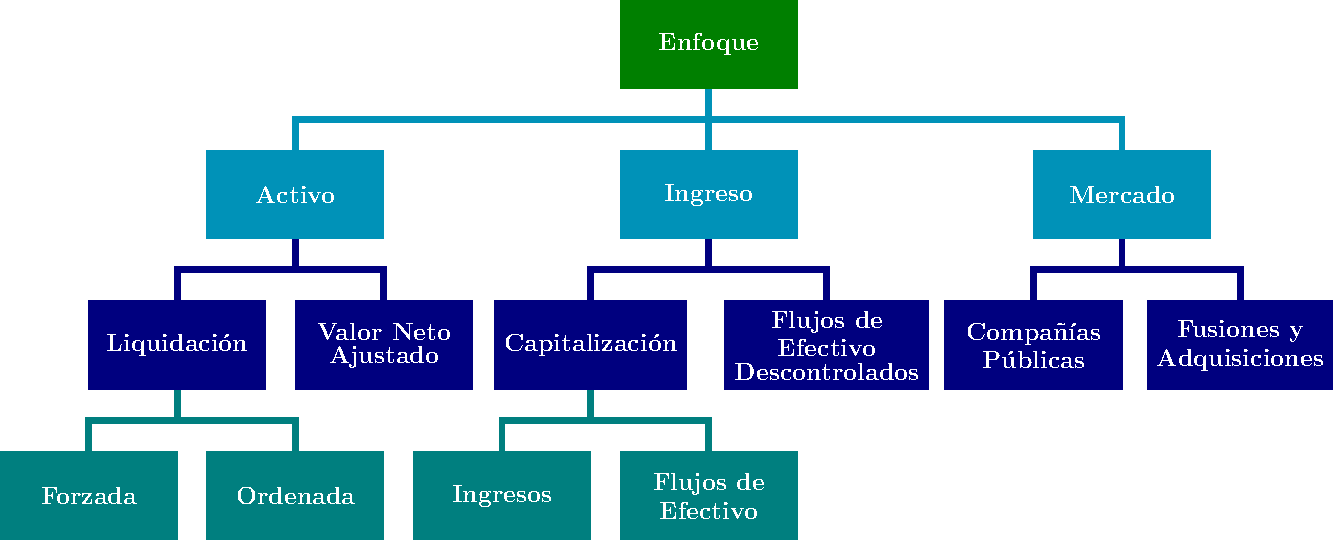
\includegraphics[width=14cm]{\rutaImagenes/enfoques_mas_utilizados_eng}
\end{figure}

\subsubsection{Asset Approach}

The asset approach is a general way to determine the fair value of a company's equity, a business, investment project, tangible asset, or intangible asset using one or more methods based on the value of assets and their net liabilities.\\[10pt]

In business valuation, the asset approach can be considered equivalent to the cost approach in other valuation disciplines. \\[10pt]

There are two general methods in the asset approach for business valuation:\\[10pt]

\textcolor{secundario}{Adjusted Book Value Method:} This method adjusts assets and liabilities (including off-balance sheet items, intangibles, and contingent liabilities) to their market value.\\[10pt]

\textcolor{secundario}{Excess Earnings Capitalization Method:} This method involves a revaluation of all the assets and liabilities of the company. This method is not used to determine the total value of a business but to determine the value of goodwill or intangible assets.\\[10pt]

It is important to distinguish between the application of a valuation method within the asset approach and the ``book value''. Under any valuation standard, the fact that the market value of a business or company is equal to its book value would be a coincidence or would depend on very particular circumstances of the entity being valued.\\[10pt]

\subsubsection{Market Approach}

The market approach determines the fair value of a company's equity, business, investment project, tangible asset, or intangible asset by using methods that compare the appraised asset with similar assets.\\[10pt]

The business, shares, tangible assets, or intangible assets used for comparison should be reasonably similar to the appraised asset. Key factors to consider in determining comparability include:\\[10pt]

\begin{itemize}

\item Sufficient similarity in quantitative and qualitative characteristics.

\item The amount and verifiability of information regarding the asset.

\item Whether the price of the similar asset was determined in a transaction between independent parties, i.e., in a voluntary sale between the parties.

\item Comparisons are generally made using valuation ratios (multiples); the calculation and use of these ratios should provide a significant reference regarding the value of the asset, considering all relevant factors.

\end{itemize}

Methods in the market approach include:\\[10pt]

\textcolor{secundario}{Public Company Guideline Method:} This method determines market multiples of stock prices of publicly traded companies (listed on a stock exchange) with a similar line of business to the appraised company.\\[10pt]

\textcolor{secundario}{Transaction Guideline Method:} This method determines market multiples of similar transactions completed between independent parties.\\[10pt]

\subsubsection{Income Approach}

The income approach is a general way to determine the fair value of a company's equity, business, asset, or intangible asset using one or more methods by which economic benefits are converted into value.\\[10pt]

In the income approach, anticipated benefits are expressed in monetary terms and can be reasonably represented by concepts such as dividends or distributions, various types of earnings, or cash flows.\\[10pt]

To estimate anticipated benefits, elements such as capital structure, historical performance of the entity, the future industry environment, and economic factors must be considered.\\[10pt]

Anticipated benefits are converted into value through procedures that consider expected growth and timing of benefits, as well as the risk profile of the benefits and the time value of money.\\[10pt]

Typically, converting anticipated benefits into value requires determining a capitalization rate or discount rate. To determine these rates, factors such as interest rate levels, expected rates of return by investors in alternative investments, and specific risk characteristics of anticipated benefits must be considered.\\[10pt]







\espacio{7cm}
%	\begin{center}
	\underline{\textbf{\textcolor{principal}{ACR\'ONIMOS}}}
\end{center}

\begin{table}[H]
 	\begin{tabular}{rp{10cm}}
\textit{Beta}:&	El coeficiente Beta ($\beta$) es una medida de volatilidad que estima el riesgo sistem\'atico de un activo.\\
\textit{CAGR}:&	Tasa compuesta de crecimiento anual.\\
\textit{CAPM}:&	Modelo de valoraci\'on de Activos de Capital.\\
\textit{Cash \& Eq.}:&	Efectivo y Equivalentes.\\
\textit{DCF}:&	Flujo de efectuvo descontado, siglas de \textit{Discounted Cash Flow}.\\\textit{Effective Tax Rate:}&	Tasa fiscal efectiva.\\
\textit{Enterprise value}:&	Valor de la empresa.\\
\textit{Equity value}:&	Valor del capital accionario.\\
\textit{Exp. Debt}:& 	Deuda expl\'icita.\\
\textit{ERP}:	& Premio de mercado.\\
\textit{Fair Value}:&	Valor razonable o valor justo de mercado.\\
\textit{FCFF}:&	Flujo de efectivo libre a la Firma, siglas de \textit{Free Cash Flow to Firm}.\\
\textit{Firm value}:&	Valor de la firma o empresa.\\
\textit{Growth Rate (G):}&	Tasa de Crecimiento de ingresos netos.\\
\textit{Income Statemen}t:&	Estado de Resultados.\\
\textit{Investment Capital}:& 	Capital Invertido (IC).\\
\textit{Ke}:& 	Costo del Capital Accionario.\\
\textit{Kd}:& 	Costo de la deuda.\\
%\textit{KPI}:&	Indicador clave de desempe\~no o indicadores de gesti\'on (\textit{Key Performance Indicator}).\\
\textit{Levered beta}:& 	Beta apalancada.\\
\textit{Market approach}:& 	Enfoque de mercado.\\
\textit{MPEEM}:&	Multi-Period Excess Earnings Method.\\
\textit{NCA}:&	Activo No Corriente.\\
\textit{Net Debt}:& 	Deuda neta.\\
\textit{Nopat}:& 	Flujo de Operaci\'on Neto.\\
\textit{NWC}:&	Capital de Trabajo Neto.\\
\textit{PEERS}:&	M\'ultiplos de Cotizaci\'on.\\
\textit{RFR}:& M\'etodo de Flujo de Ahorro en Regal\'ias\\
\textit{Risk free rate}:&	  Tasa Libre de Riesgo.\\
%\textit{Size prime}:&	Prima por tama\~no.\\
\textit{Terminal value}:&	Valor terminal.\\
\textit{Total Debt}:&	Deuda total.\\
\textit{Value drivers}:&  	Elevadores de Valor.\\
\textit{WACC}:& 		Costo Promedio Ponderado de Capital.\\
\textit{WARA}:&	 Costo Promedio Ponderado de Activos.\\


	\end{tabular}
\end{table}
%	
%	\begin{center}
% 	\printnoidxglossary[type=\acronymtype,title={Acr\'onimos}]
%	\printnoidxglossary
%	\end{center}
	
	
\chapter{METODOLOG\'IA DE VALUACI\'ON.}\label{cap:4}
\thispagestyle{fancy}

Se llev\'o a cabo la valuaci\'on del bien mencionado en el \autoref{cap:2} inciso \autoref{sec:f} de este informe; mismo que se explica a continuaci\'on:

%-----------------------Descripci\'on de los enfoques de valuaci\'on aplicados-------------
\setcounter{section}{10}
\section{DESCRIPCI\'ON DE LOS ENFOQUES DE VALUACI\'ON APLICADOS.}\label{sec:k}

\renewcommand\thefigure{\arabic{figure}} 

Para la emisi\'on del presente dictamen, se aplic\'o el m\'etodo comparativo referencial directo, atendiendo a la comparaci\'on de obras del mismo autor, t\'ecnica, calidad y medidas similares.
3\\
\begin{enumerate}[a.]
\item Enfoque de Mercado: comparaci\'on de ventas realizadas en ofertas similares con el objeto de deducir el precio m\'as probable que podr\'ia alcanzar el bien valuado.

\item \'Indice de afectaci\'on real: factores extr\'insecos del bien que influyen directamente el valor de la obra.

\item Valor de Mercado: es ``el monto estimado por el que se intercambiar\'ia un activo a la fecha de la valuaci\'on entre un vendedor y un comprador dispuestos en una transacci\'on independiente, despu\'es de una adecuada promoci\'on, donde las partes act\'uan con conocimiento, de forma prudente y sin compulsi\'on.'' (Fuente: \textit{International Valuation Standards Council}).

\item Valor comercial: precio m\'as probable que tendr\'ia un bien a la fecha de emisi\'on del aval\'uo.

\end{enumerate}



\chapter{DESARROLLO DE LA VALUACI\'ON}\label{cap:5}
\thispagestyle{fancy}

%-----------------------Desarrollo del avalúo en la especie------------------------------------
\setcounter{section}{11}

\subsection{DESARROLLO DEL AVAL\'UO EN LA ESPECIE.}\label{sec:k2}

\subsubsection{An\'alisis Financiero}
\begin{enumerate}[1.]

\item Sobre el artista.\\
\insertar

\item T\'ecnica:

Grafito sobre papel hecho a mano.

\item Estilo:

Dibujos en grafito en tonalidades grises, negro. Tema fant\'astico, mitol\'ogico, combinaci\'on de figuras sobrenaturales. \\

Representaci\'on de arte precolombino, im\'agenes de deidades, figuras antropomorfas, cabezas colosales, culto religioso indígena y personajes mitol\'ogicos.\\

\item M\'etodo comparativo referencial directo:
\begin{enumerate}[a.]

\item En cuanto al valor de Mercado del artista a quien se le atribuye la obra:\\

No se encontraron antecedentes de la comercializaci\'on de obras atribuidas al Arquitecto Arq. Ra\'ul Gonz\'alez Esquivel.

\item En cuanto a la firma del autor a quien se le atribuye la obra:

En la parte inferior derecha de las obras, se presenta la firma plasmada con diversas fechas, de las que se desprende que la composici\'on, el trazado y la diagramaci\'on, as\'i como el tama\~no, la forma, la direcci\'on, la inclinaci\'on, la presi\'on, el espacio y la velocidad del trazado de la firma, es notoriamente similar en todas las obras objeto de valuaci\'on. A continuaci\'on se muestran muestras aleatorias:

\begin{figure}
\centering
\includegraphics[width=\textwidth]{../0.imagenes/firmas}
\end{figure}

Adicionalmente, se reitera que Licenciado Carlos Campos Echeverr\'ia cuenta con certificado de autenticidad de las obras emitido por Pablo C. Goebel, de los que se desprende que la autor\'ia de las obras objeto de valuaci\'on, se atribuye al Arquitecto Ra\'ul Gonz\'alez Esquivel.
\end{enumerate}

\item Elementos de estudio:

\begin{enumerate}[a.]

\item Inspecci\'on ocular de la obra.

\item B\'usqueda de antecedentes registrales y comerciales del artista. 
\item Estudio de mercado en Galer\'ias, Casas de subasta. An\'alisis comparativo.

\item Factores de \'indice de afectaci\'on real:

\end{enumerate}

\item Valor de Mercado:

Considerando el m\'etodo comparativo referencial directo y los factores de \'indice de afectaci\'on real, as\'i como los elementos de prueba y alcance del trabajo valuatorio realizado por el suscrito, se concluye que el valor estimado de Mercado de las obras objeto del presente dictamen, es de \insertar, en t\'erminos de lo siguiente:\\

\insertar

\end{enumerate}





\espacio{1cm}

%-----------------------FECHA DE INSPECCIÓN---------------------
\section{FECHA DE INSPECCI\'ON}\label{sec:l}
\fechaInspeccion.

%------------------------FECHA DE VALORES------------------------
\section{FECHA DE VALORES}\label{sec:m}
Fecha de valores al \fechaValores.

%-----------------------FECHA DEL INFORME-----------------------
\section{FECHA DEL INFORME}\label{sec:n}
Fecha del informe, \fechaInforme.

%----------------------FUENTES DE INFORMACIÓN--------------
\section{FUENTES DE INFORMACI\'ON}\label{sec:nn}
\begin{itemize}
	\begin{itemize}

\item To obtain economic data for Mexico such as inflation, please consult the website of the National Institute of Statistics and Geography (INEGI): \url{http://www.inegi.org.mx/sistemas/IndicePrecios/}

\item For financial information related to industry, sector, discount rates, and peers, you can visit: \url{https://www.refinitiv.com/en}

\item To access reference data on risk-free rates for Mexico, please refer to the website of the Bank of Mexico: \url{www.banxico.org.mx}

\item For obtaining macroeconomic indicators, you can find information from ``Economía en breve'' by Mtro. Mario Correa at: \url{https://www.youtube.com/channel/UCtt93euOsTuq_gjUiZV-MSA}

\item For other financial data, you can visit the following websites:
\begin{itemize}
\item\url{www.damodaran.com}
\item \url{www.reuters.com}
\item \url{www.bmv.com.mx}
\item \url{www.sat.gob.mx}
\end{itemize}

\item For sector analysis, brand profiles, and the macro environment, you can access Passport Euromonitor at: \url{https://www.portal.euromonitor.com/}
\begin{itemize}
\item \url{https://www.vivo.com/en}
\item \url{https://www.vivo.com/mx}
\item \url{https://www.statista.com/statistics/541618/vivo-smartphone-shipments-worldwide/}
\item Vivo share of global smartphone shipments 2019-2023. Statista
\item Vivo Communication Technology. Crunchbase Company Profile \& Funding
\item La venta de ``smartphones'' mueve 93.000 millones hasta marzo: qué marcas suben y cuál se desploma? \url{elpais.com}
\end{itemize}
	 
\end{itemize}
	%\fuentes
\end{itemize}
%-----------------------CONSIDERACIONES PREVIAS A LA CONCLUSI\'ON------------------
\section{CONSIDERACIONES PREVIAS A LA CONCLUSI\'ON}\label{sec:o}
\begin{enumerate}
	\item El presente estudio s\'olo es v\'alido para el prop\'osito y uso que se indica en los incisos \ref{proposito} e \ref{uso} de este dictamen y cuando cuente con la firma \ifthenelse{\equal{\peritoAuxiliar}{n/a}}{del perito valuador}{de los peritos valuadores}.
	\item Las declaraciones de hechos, datos y documentos proporcionados por el solicitante para la realizaci\'on de este informe, se asumen como verdaderas y correctas.
	\item El an\'alisis y opiniones reportados en el presente dictamen est\'an limitados s\'olo por las suposiciones y condiciones limitantes reportadas y son el resultado de las conclusiones profesionales e imparciales  \ifthenelse{\equal{\peritoAuxiliar}{n/a}}{del valuador que firma}{de los valuadores que firman}.
	\item  \ifthenelse{\equal{\peritoAuxiliar}{n/a}}{El perito valuador que firma no tiene}{Los peritos valuadores que firman no tienen}{} inter\'es presente o futuro en las cifras conclusivas de las que es objeto de este informe, ni tampoco  \ifthenelse{\equal{\peritoAuxiliar}{n/a}}{tiene}{tienen}{} intereses personales o parcialidad con respecto a las partes involucradas.
	\item La compensaci\'on econ\'omica  \ifthenelse{\equal{\peritoAuxiliar}{n/a}}{del perito valuador}{de los peritos valuadores}{} no est\'a condicionada al informe de un valor predeterminado o dirigido a un valor que favorezca la causa del solicitante.
	\item Este dictamen valuatorio s\'olo podr\'a ser usado \'integro y no en partes. Ninguna parte del reporte podr\'a ser utilizada en conjunto a alg\'un estudio ajeno al mismo. La publicaci\'on del mismo o cualquiera de sus partes, sin la autorizaci\'on escrita del suscrito Corredor P\'ublico est\'a prohibida. Este aval\'uo no podr\'a ser usado por ninguna persona o entidad distinta a la que est\'e dirigida o para un prop\'osito o fin distinto al estipulado.
	\item El presente estudio no valida o se\~nala el tratamiento jur\'idico, contable y/o fiscal de las cifras conclusivas del informe; conforme a las normas de informaci\'on financiera (NIF), la ley del ISR, la Ley del IVA y dem\'as normatividad aplicable.

\end{enumerate}

\espacio{7cm}
\chapter{CONCLUSIONES.}\label{cap:6}
\thispagestyle{fancy}
%-----------------------CONCLUSIÓN DE LA VALUACIÓN-----------------------
\setcounter{section}{16}
\section{CONCLUSI\'ON DE LA VALUACI\'ON.}\label{sec:p}

Sobre el valor de Mercado de la obra art\'istica se concluye:

\textcolor{principal}{\underline{PRIMERA.-}} La emisi\'on del presente dictamen valuatorio no representa un certificado de autenticidad de la obra objeto de valuaci\'on, por lo que su emisi\'on, distribuci\'on y/o reproducci\'on, de manera alguna puede entenderse como certificado de autenticidad y/o t\'itulo de propiedad del solicitante.\\



\textcolor{principal}{\underline{SEGUNDA.-}} El valor estimado de Mercado de las obras objeto de dictamen es de \insertar.\\

\vspace{2cm}

A nuestro mejor juicio y parecer, siendo los \textcolor{principal}{ \diainforme{} d\'ias del mes de \monthname[\mesinforme]{} del a\~no \annoinforme{} (\numberstringnum{\annoinforme})} seg\'un el criterio valuatorio explicado en el desarrollo de este dictamen, expedimos el presente \textcolor{principal}{DICTAMEN VALUATORIO}, con \textcolor{principal}{\textbf{FECHA DE VALORES}} al d\'ia \textcolor{principal}{\textbf{\fechaValores}}; para todos los efectos a que haya lugar.\\

Por todo lo cual y con fundamento en el artículo 6$^\circ$ fracción II de la Ley Federal de Correduría Pública y el artículo 56 bis de su Reglamento, para los efectos legales a que hubiera lugar, rindo el presente avalúo y lo expido debidamente en la Ciudad de México, hoy día de su fecha, \diainforme{}  (\numberstringnum{\diainforme}) de \monthname[\mesinforme] de \annoinforme (\numberstringnum{\annoinforme}).



\begin{table}[H]
\centering
	\begin{tabular}{cm{1cm}c}
	\begin{minipage}{7cm}
	\begin{center}
		JOSÉ RAMÓN CLARK GUZMÁN,
		Corredor Público número 81 de la
		Ciudad de México, expido el presente
		dictamen valuatorio.\\[1cm]
		
		\rule{7cm}{.4pt}\\
		JOSÉ RAMÓN CLARK GUZMÁN
		
		
	\end{center}
	\end{minipage}&&
	\begin{minipage}{7cm}
	\begin{center}
		PERITO AUXILIAR\\[1cm]
		
		\rule{7cm}{.4pt}\\
		DIEGO MIGUEL\\
		PEREZCANO BELTRÁN
		%\nombreAuxiliar\\
		%\textcolor{principal}{\descripcionFirmaAuxiliar}
		
	\end{center}
	\end{minipage}
	
	\end{tabular}
\end{table}


%----------------------REPORTE FOTOGRAFICO------------------------------
\section{REPORTE FOTOGR\'AFICO}\label{sec:q}
No Aplica.
%---------------------ANEXOS-------------------------------------------------------- 
\section{ANEXOS}\label{sec:r}

\newpage


\label{lastpage}
\end{document}
